\documentclass[12pt,a4paper]{article}

\usepackage[a4paper,margin=1in]{geometry}
\usepackage{graphicx}
\usepackage{booktabs}
\usepackage{amsmath,amssymb}
\usepackage{float}
\usepackage{hyperref}
\usepackage{xcolor}
\usepackage{listings}
\usepackage{enumitem}
\usepackage{fancyhdr}
\usepackage{longtable}

\hypersetup{colorlinks=true,linkcolor=blue,urlcolor=blue}

\pagestyle{fancy}
\fancyhf{}
\lhead{ICS1512}
\rhead{Machine Learning Algorithms Laboratory}
\cfoot{\thepage}

\lstset{
language=Python,
basicstyle=\ttfamily\small,
numbers=left,
frame=single,
breaklines=true,
showstringspaces=false,
keywordstyle=\color{blue}\bfseries,
commentstyle=\color{teal}\itshape,
stringstyle=\color{red}
}

\begin{document}

\begin{tabular}{|p{4cm}|p{11cm}|}
\hline
Experiment No. & 1 \\ \hline
Experiment Title & Universal Exploratory Data Analysis, Data Preprocessing, and Feature Engineering across Python Scientific Packages \footnote{\textbf{GitHub Repository: }\url{https://github.com/Kavin-ks/Machine-Learning-Projects}}\\ \hline
Student Name & Kavinsoorya K S \\ \hline
Register Number & 3122247001030 \\ \hline
Faculty & Dr. Poreddy Ajay Kumar Reddy \\ \hline
Submission Date & July 25, 2026 \\ \hline
\end{tabular}

\vspace{0.5cm}

\section{Objective}
The objective of this experiment is to explore Python scientific computing and data analysis libraries (\texttt{NumPy}, \texttt{Pandas}, \texttt{SciPy}, \texttt{Scikit-Learn}, \texttt{Matplotlib}, and \texttt{Seaborn}) to perform automated Exploratory Data Analysis (EDA), feature selection, data preprocessing, baseline model fitting, and comparative performance evaluation across five benchmark machine learning datasets.

\section{Problem Statement}
In machine learning workflows, raw datasets differ significantly in feature dimensionality, scale, data types, missingness, and problem domains (tabular classification, continuous regression, unstructured text mining, medical diagnosis, and computer vision). To establish robust predictive models, an automated data processing and analytical pipeline must be developed to identify task types, inspect distributions, impute noise, extract relevant features, partition datasets into train-test splits, fit baseline machine learning algorithms, and quantify evaluation metrics.

\section{Universal EDA Architecture (\texttt{perform\_EDA})}
To standardize exploratory analysis across diverse data formats, a reusable Python function \texttt{perform\_EDA()} was constructed in \texttt{universal\_eda.ipynb}. The complete code implementation is provided below:

\begin{lstlisting}[caption={Complete Universal EDA Implementation Code (perform\_EDA)}]
import pandas as pd
import numpy as np
import matplotlib.pyplot as plt
import seaborn as sns
from scipy import stats

def perform_eda(file_path):
    """
    Universal EDA (Stops before preprocessing/modeling)

    Works for:
    Iris, Loan, Diabetes, MNIST(CSV), Spam(SMS)

    Usage:
        perform_eda("file.csv")
    """

    try:
        df = pd.read_csv(file_path, encoding="latin1")
    except Exception:
        df = pd.read_csv(file_path)

    print("="*80)
    print("DATASET OVERVIEW")
    print("="*80)
    print("Shape :", df.shape)
    print("\nColumns\n", df.columns.tolist())
    print("\nInfo")
    df.info()
    print("\nFirst 5 Rows")
    print(df.head())
    print("\nSummary")
    print(df.describe(include="all"))
    print("\nMissing Values")
    print(df.isnull().sum())
    print("\nDuplicate Rows :", df.duplicated().sum())

    # ---------- Spam ----------
    if "v1" in df.columns and "v2" in df.columns:
        df = df.drop(columns=[c for c in df.columns if "Unnamed" in c], errors="ignore")
        df.columns = ["Label", "Message"]
        df["Length"] = df["Message"].str.len()

        #1 Countplot
        sns.countplot(data=df, x="Label")
        plt.title("Spam vs Ham")
        plt.show()

        #2 Message Length Distribution
        sns.histplot(df["Length"], kde=True)
        plt.title("Message Length Distribution")
        plt.show()

        #3 Boxplot
        sns.boxplot(data=df, x="Label", y="Length")
        plt.title("Message Length Boxplot")
        plt.show()

        #4 Violin Plot
        sns.violinplot(data=df, x="Label", y="Length")
        plt.title("Message Length Violin Plot")
        plt.show()

        #5 QQ Plot
        stats.probplot(df["Length"], dist="norm", plot=plt)
        plt.title("QQ Plot")
        plt.show()

        #6 Scatter Plot
        plt.scatter(range(len(df)), df["Length"], s=8)
        plt.title("Length Scatter")
        plt.xlabel("Message Index")
        plt.ylabel("Length")
        plt.show()

        #7 Groupby summary
        print(df.groupby("Label")["Length"].describe())
        return

    # ---------- MNIST ----------
    if "label" in df.columns and df.shape[1] == 785:

        #1 Digit Distribution Countplot
        sns.countplot(data=df, x="label")
        plt.title("Digit Distribution")
        plt.show()

        #2 Sample Grayscale Images
        plt.figure(figsize=(12, 5))
        for i in range(10):
            plt.subplot(2, 5, i+1)
            plt.imshow(df.iloc[i, 1:].values.reshape(28, 28), cmap="gray")
            plt.title(df.iloc[i, 0])
            plt.axis("off")
        plt.tight_layout()
        plt.show()

        pixels = df.iloc[:, 1:].values.flatten()

        #3 Pixel Distribution
        sns.histplot(pixels, bins=40)
        plt.title("Pixel Distribution")
        plt.show()

        #4 Pixel Boxplot
        sns.boxplot(x=pixels)
        plt.title("Pixel Boxplot")
        plt.show()

        #5 Pixel Violin Plot
        sns.violinplot(x=pixels)
        plt.title("Pixel Violin Plot")
        plt.show()

        #6 Pixel QQ Plot
        stats.probplot(pixels[:5000], dist="norm", plot=plt)
        plt.title("Pixel QQ Plot")
        plt.show()

        #7 Value counts
        print(df["label"].value_counts())
        return

    # ---------- Diabetes Audit ----------
    if "Outcome" in df.columns:
        cols = ["Glucose", "BloodPressure", "SkinThickness", "Insulin", "BMI"]
        print("\nPossible Missing Values Stored as Zero")
        for c in cols:
            if c in df.columns:
                print(f"{c}: {(df[c]==0).sum()}")

    num = df.select_dtypes(include=np.number).columns.tolist()
    cat = df.select_dtypes(exclude=np.number).columns.tolist()

    #1 Histograms
    for c in num:
        sns.histplot(df[c], kde=True, bins=30)
        plt.title(f"Histogram - {c}")
        plt.show()

    #2 Boxplots
    for c in num:
        sns.boxplot(x=df[c])
        plt.title(f"Boxplot - {c}")
        plt.show()

    #3 Violin Plots
    for c in num:
        sns.violinplot(x=df[c])
        plt.title(f"Violin - {c}")
        plt.show()

    #4 Countplots for Categorical
    for c in cat:
        sns.countplot(data=df, x=c)
        plt.xticks(rotation=45)
        plt.title(f"Countplot - {c}")
        plt.tight_layout()
        plt.show()

    #5 Correlation Heatmap
    if len(num) > 1:
        sns.heatmap(df[num].corr(), annot=True, cmap="coolwarm", fmt=".2f")
        plt.title("Correlation Heatmap")
        plt.show()

    #6 Pairplots
    if len(num) <= 8:
        hue = None
        for h in ["Species", "species", "Loan_Status", "Outcome"]:
            if h in df.columns:
                hue = h
                break
        sns.pairplot(df, hue=hue)
        plt.show()

    #7 Normal Probability (QQ) Plots
    for c in num:
        stats.probplot(df[c].dropna(), dist="norm", plot=plt)
        plt.title(f"QQ Plot - {c}")
        plt.show()

    print("\nEDA Completed.")
\end{lstlisting}

\section{Case Study 1: Iris Dataset}

\subsection{Dataset Description \& ML Task}
The Iris dataset contains morphometric measurements of three species of iris flowers (\textit{Iris-setosa}, \textit{Iris-versicolor}, and \textit{Iris-virginica}). The objective is a \textbf{Multiclass Classification} task to classify flower species based on four continuous physical attributes.

\subsection{Dataset Characteristics \& Summary Statistics}
\begin{itemize}
    \item \textbf{Total Samples:} 150 instances (50 per species, perfectly balanced).
    \item \textbf{Feature Dimensionality:} 4 numerical predictor features (\texttt{SepalLength}, \texttt{SepalWidth}, \texttt{PedalLength}, \texttt{PedalWidth}) and 1 target class (\texttt{Species}).
    \item \textbf{Missing Values:} 0 null values across all attributes.
    \item \textbf{Summary Statistics:} \texttt{SepalLength} (Mean: $5.84$ cm, Std: $0.83$), \texttt{SepalWidth} (Mean: $3.05$ cm, Std: $0.43$), \texttt{PedalLength} (Mean: $3.76$ cm, Std: $1.76$), \texttt{PedalWidth} (Mean: $1.20$ cm, Std: $0.76$).
\end{itemize}

\subsection{Exploratory Data Analysis}

\begin{figure}[H]
\centering
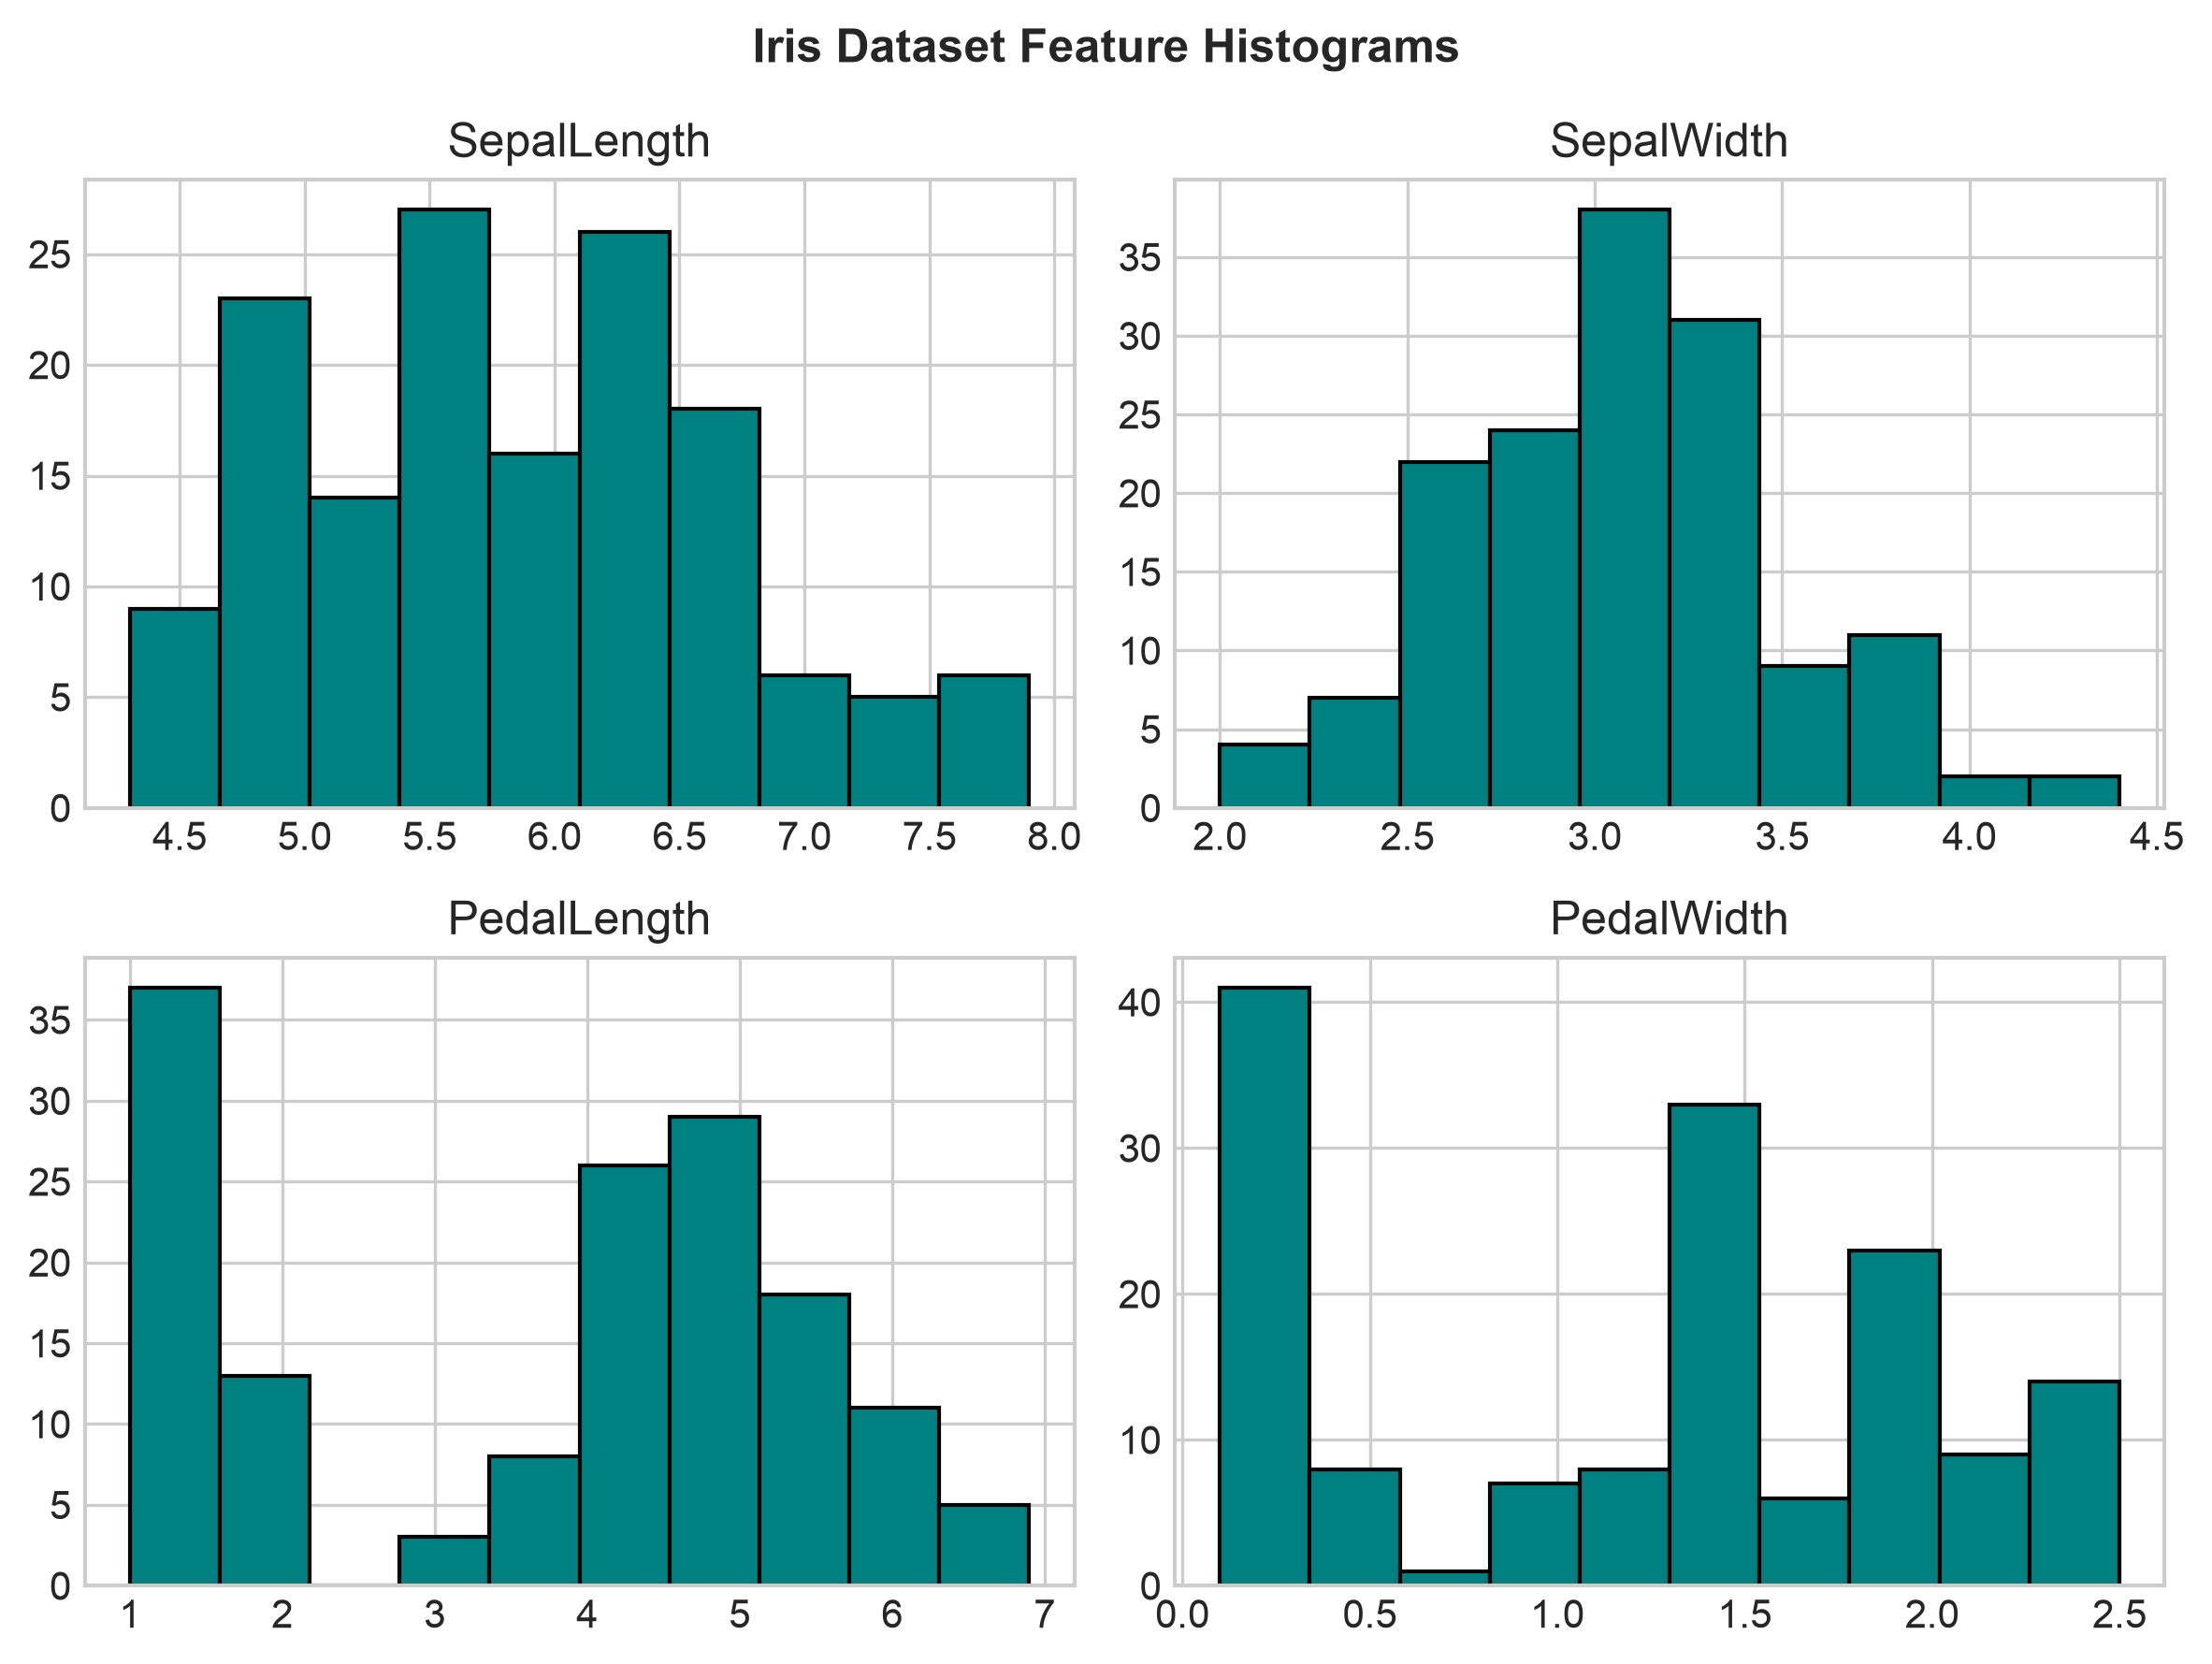
\includegraphics[width=0.75\linewidth]{images/iris_histograms.png}
\caption{Histograms of Iris Physical Measurements}
\label{fig:iris_hist}
\end{figure}

\textbf{Inference:}
\texttt{PedalLength} and \texttt{PedalWidth} display prominent bimodal distributions, separating \textit{Iris-setosa} from the remaining species, whereas \texttt{SepalLength} and \texttt{SepalWidth} follow normal bell-shaped curves.

\begin{figure}[H]
\centering
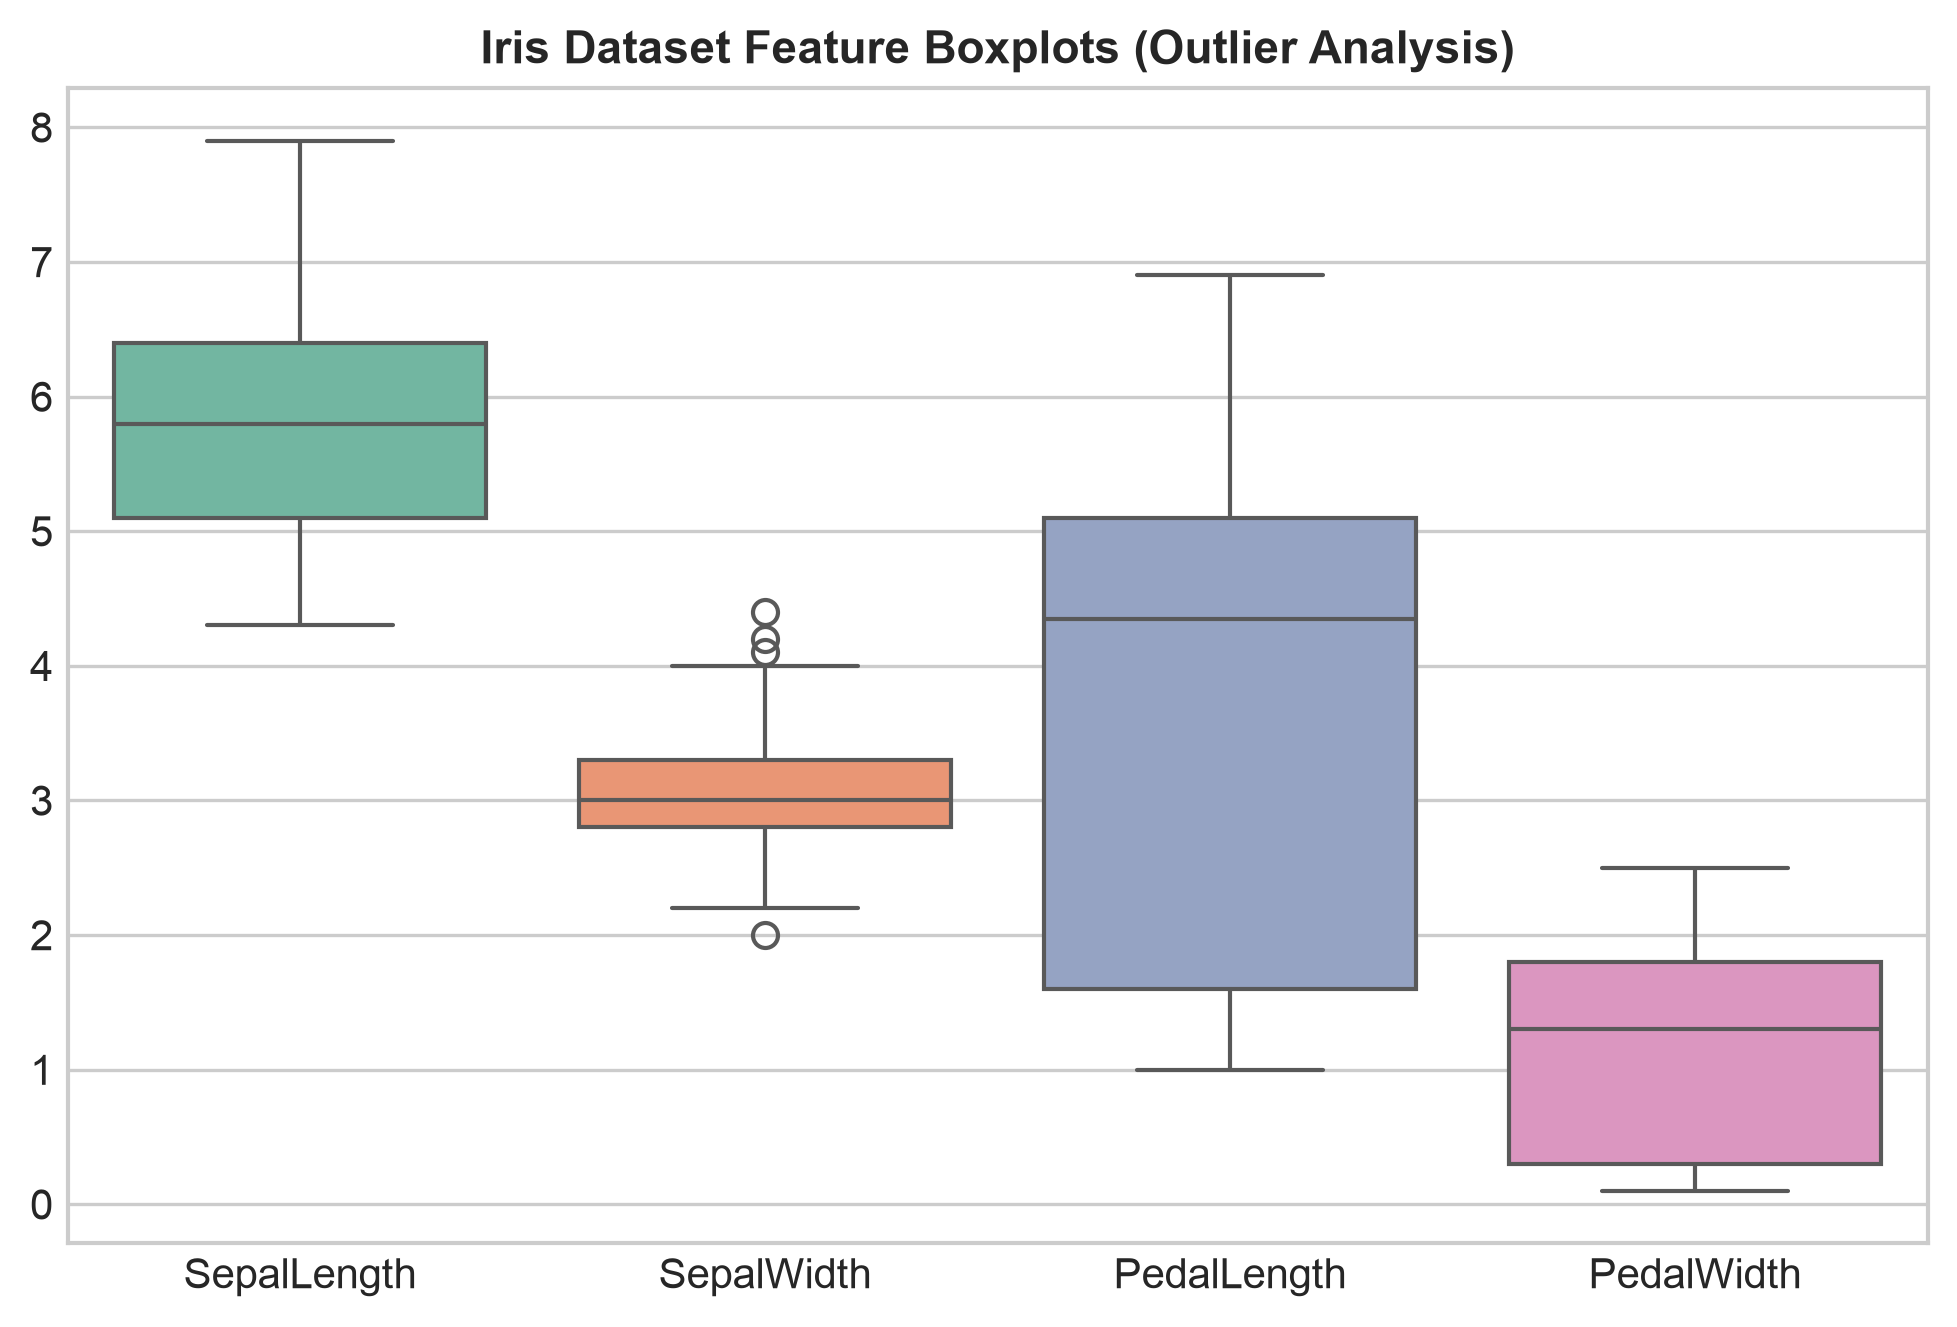
\includegraphics[width=0.75\linewidth]{images/iris_boxplots.png}
\caption{Feature Boxplots for Outlier Inspection}
\label{fig:iris_box}
\end{figure}

\textbf{Inference:}
Boxplots confirm that \texttt{PedalLength} and \texttt{PedalWidth} possess zero extreme outliers. Minor upper and lower outliers exist in \texttt{SepalWidth} around values $< 2.0$ cm and $> 4.0$ cm.

\begin{figure}[H]
\centering
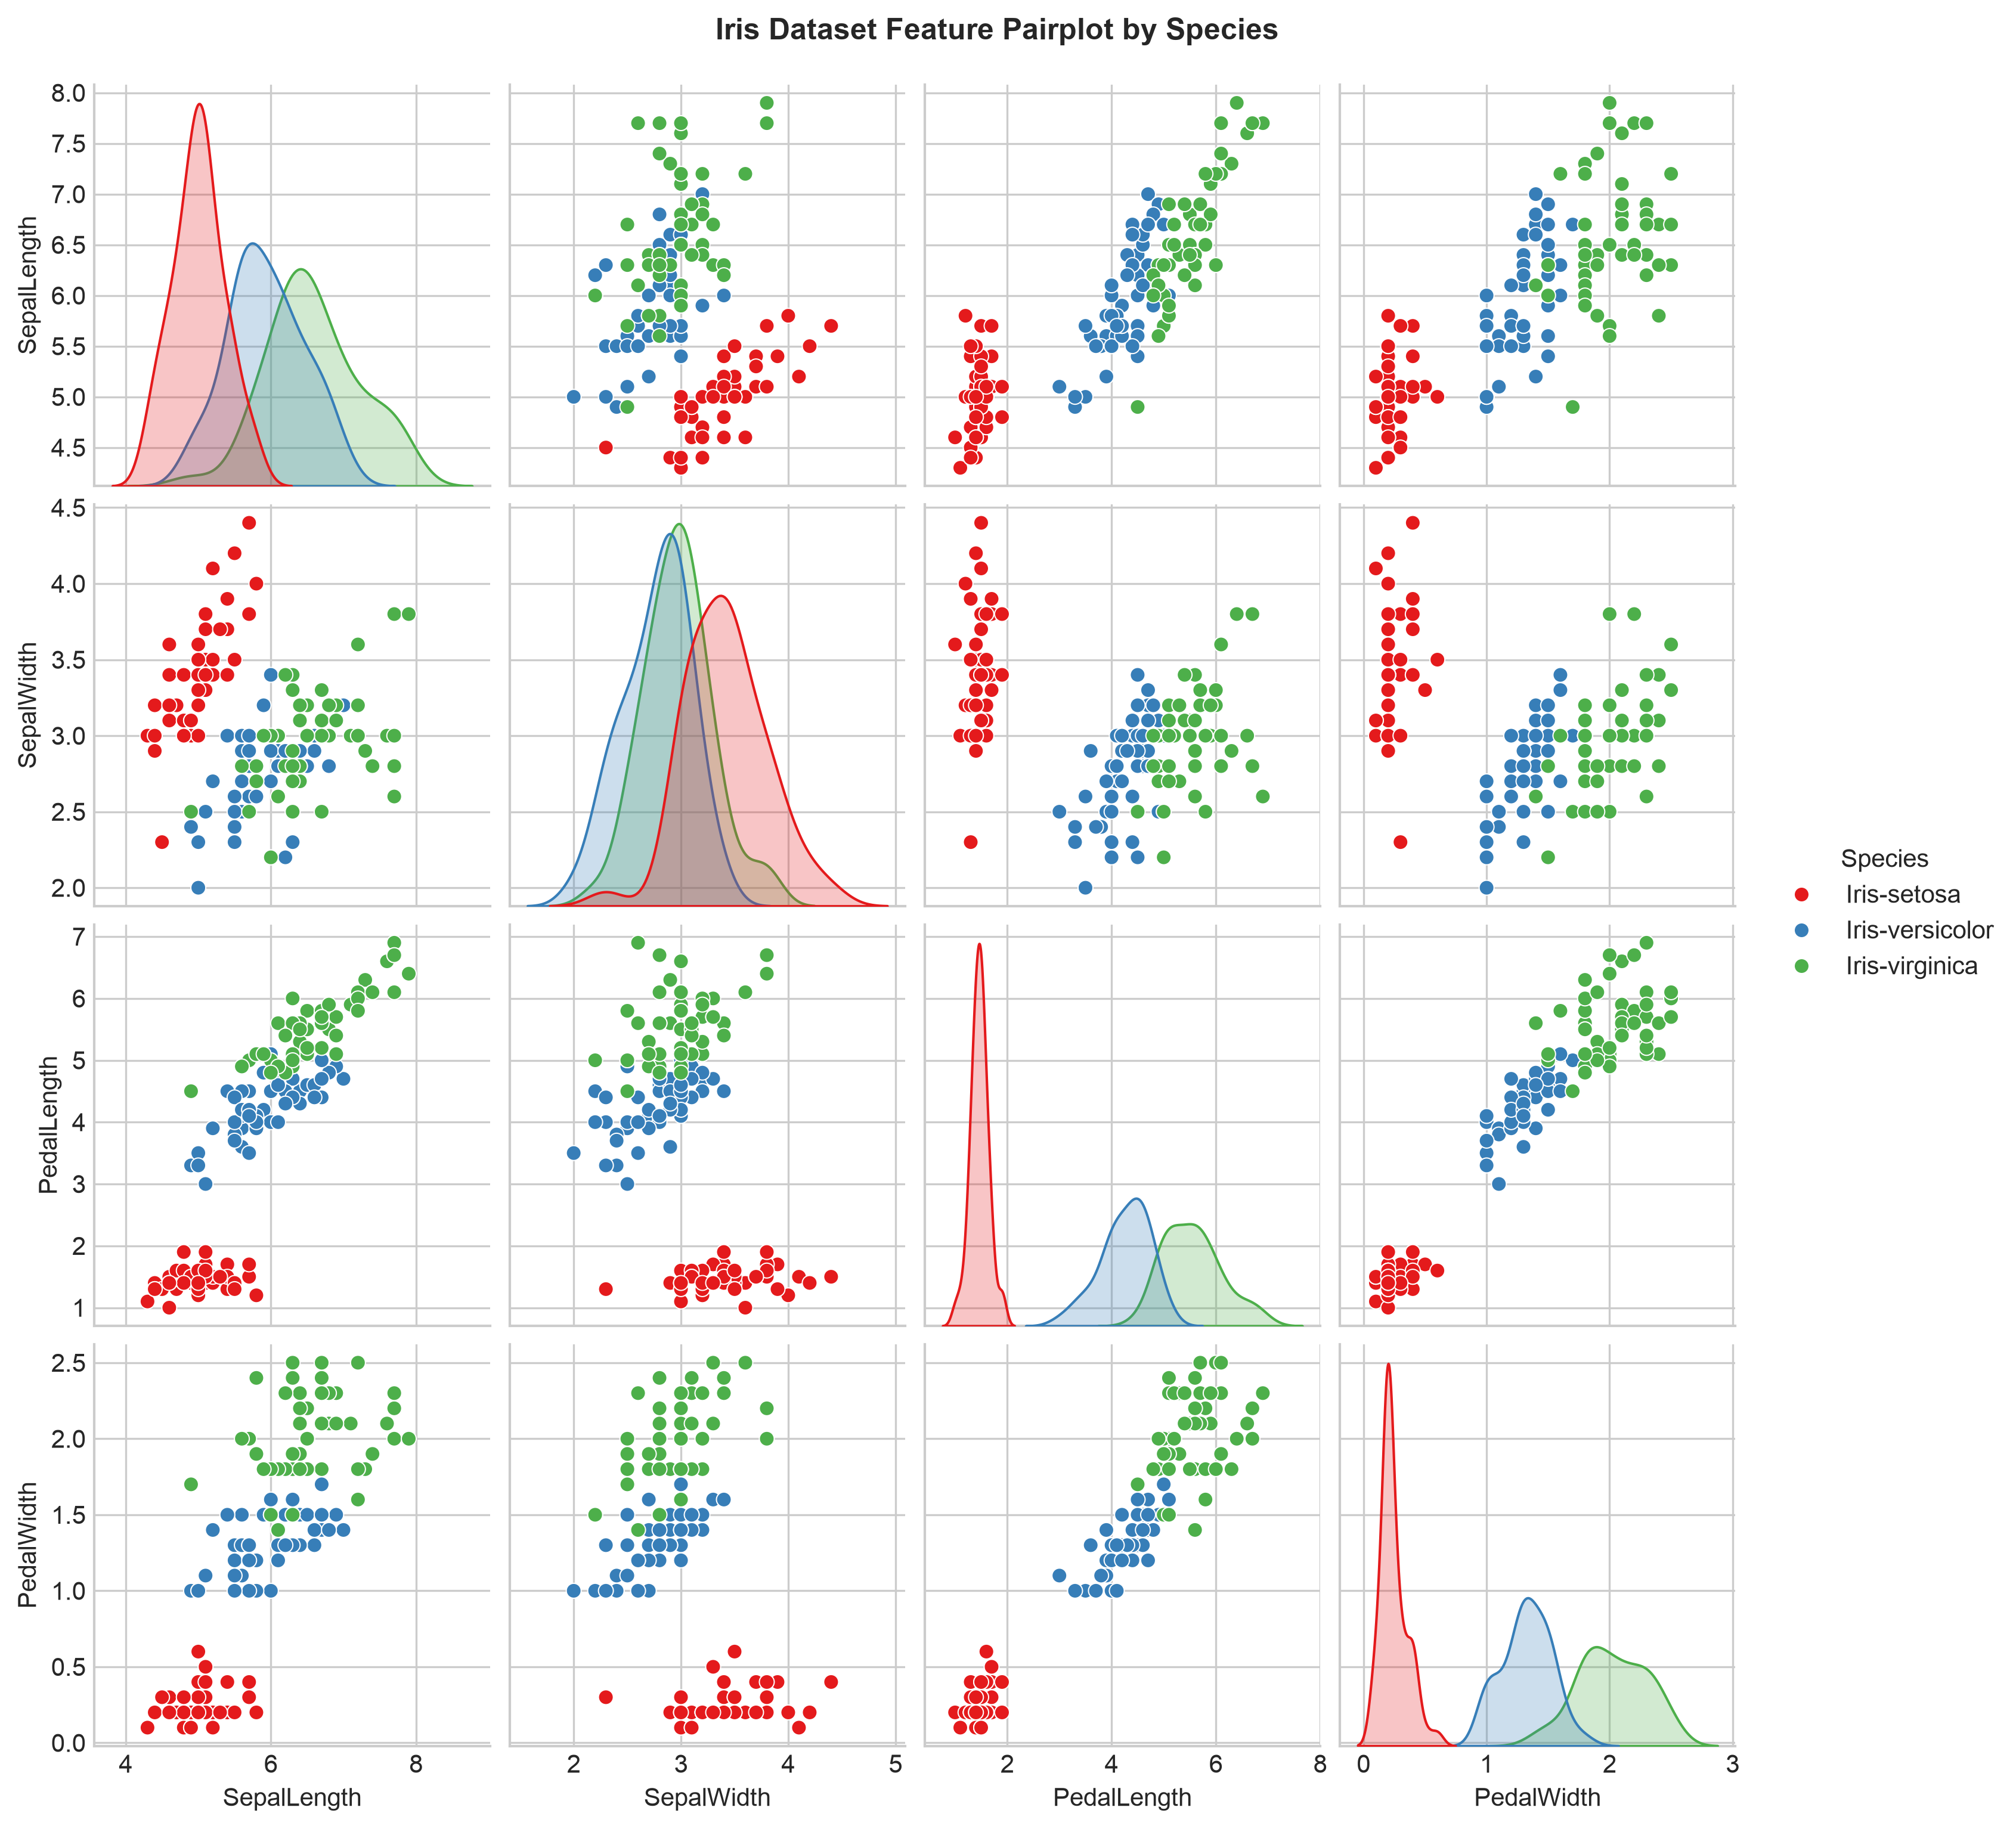
\includegraphics[width=0.75\linewidth]{images/iris_pairplot.png}
\caption{Pairplot of Iris Features Segmented by Species}
\label{fig:iris_pair}
\end{figure}

\textbf{Inference:}
\textit{Iris-setosa} is completely linearly separable from \textit{Iris-versicolor} and \textit{Iris-virginica} when plotting \texttt{PedalLength} versus \texttt{PedalWidth}. Moderate overlap exists between versicolor and virginica.

\begin{figure}[H]
\centering
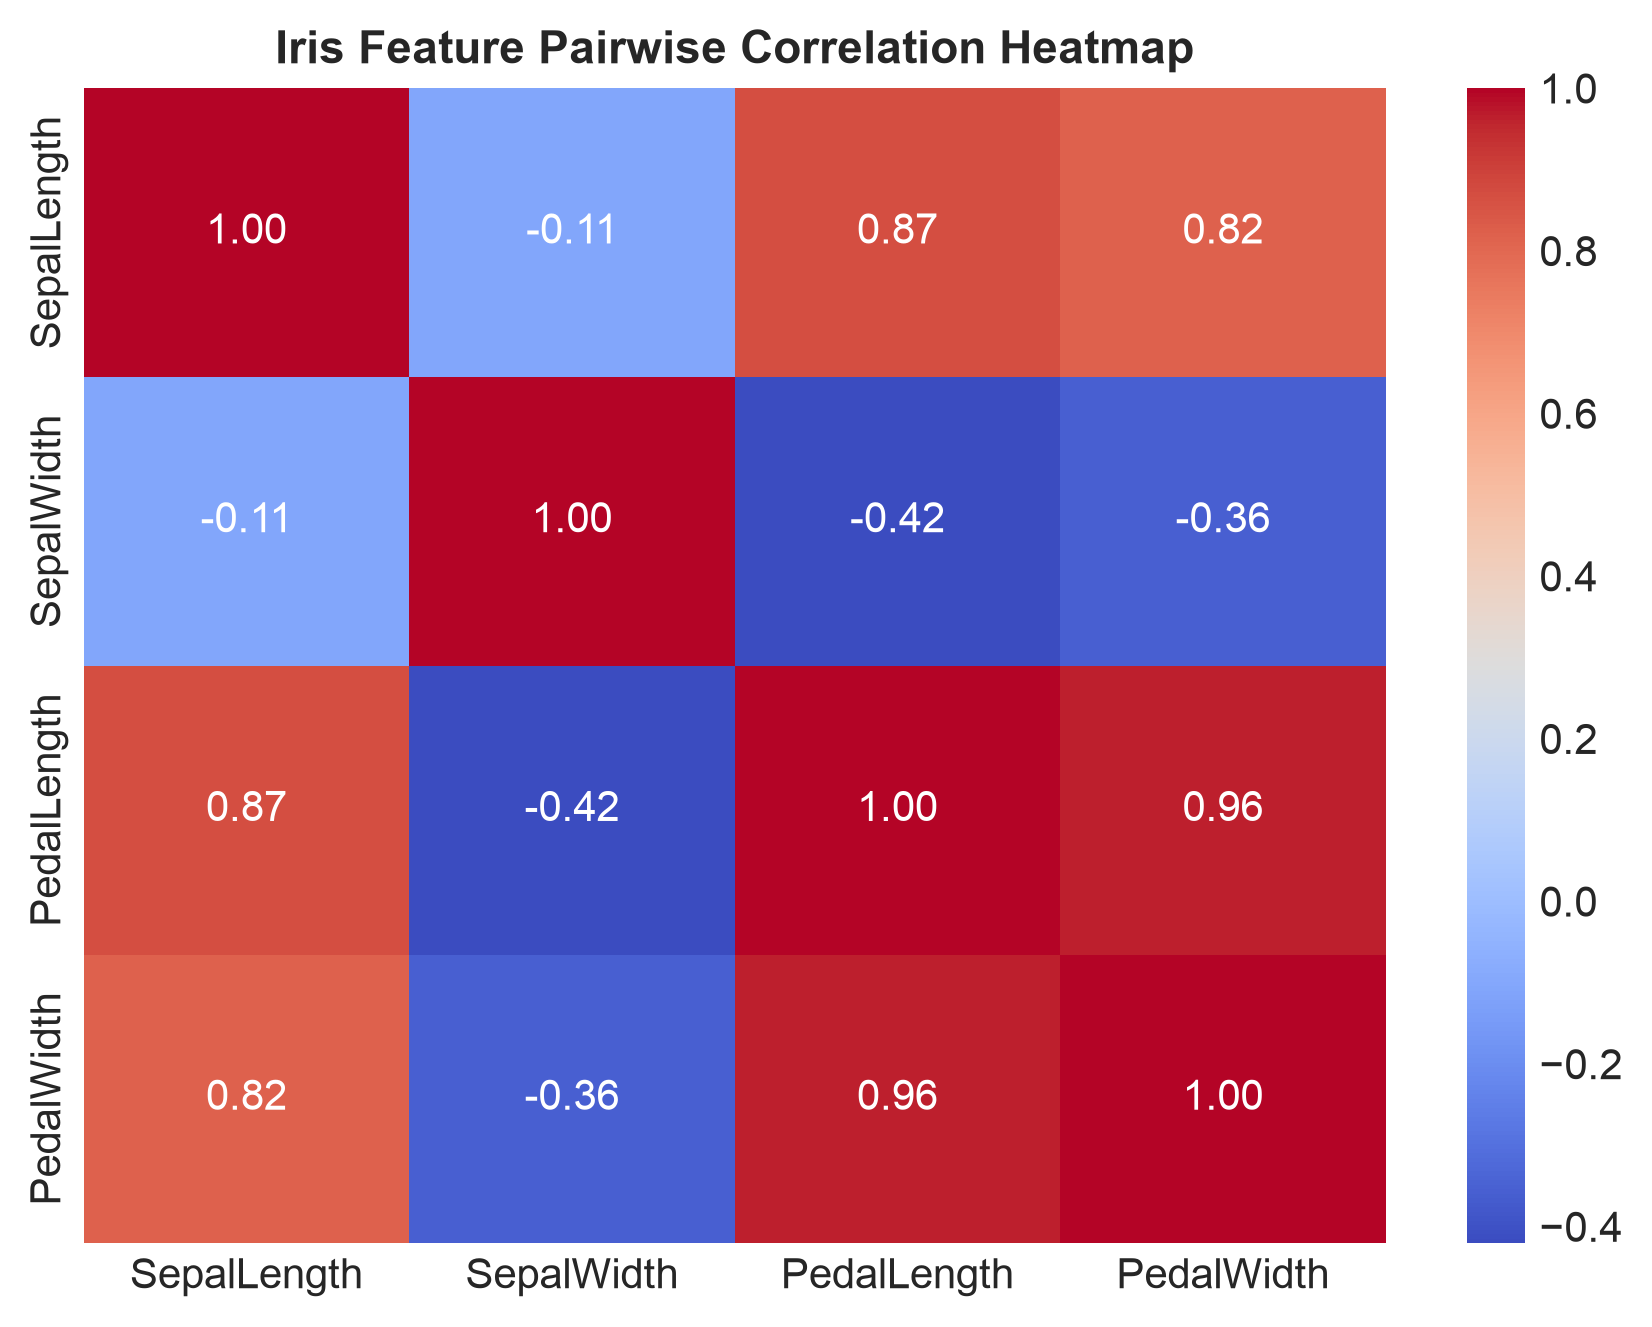
\includegraphics[width=0.65\linewidth]{images/iris_correlation.png}
\caption{Pairwise Correlation Heatmap for Iris Features}
\label{fig:iris_corr}
\end{figure}

\textbf{Inference:}
Strong positive correlation exists between \texttt{PedalLength} and \texttt{PedalWidth} ($r = 0.96$), as well as between \texttt{SepalLength} and \texttt{PedalLength} ($r = 0.87$).

\subsection{Data Preprocessing \& Model Evaluation}
\begin{itemize}
    \item \textbf{Train-Test Split:} Partitioned 80\% training ($n=120$) and 20\% testing ($n=30$).
    \item \textbf{Model Trained:} \texttt{DecisionTreeClassifier(random\_state=42)}.
    \item \textbf{Accuracy Score:} \textbf{1.0000} (100.0\% Test Accuracy).
\end{itemize}

\begin{figure}[H]
\centering
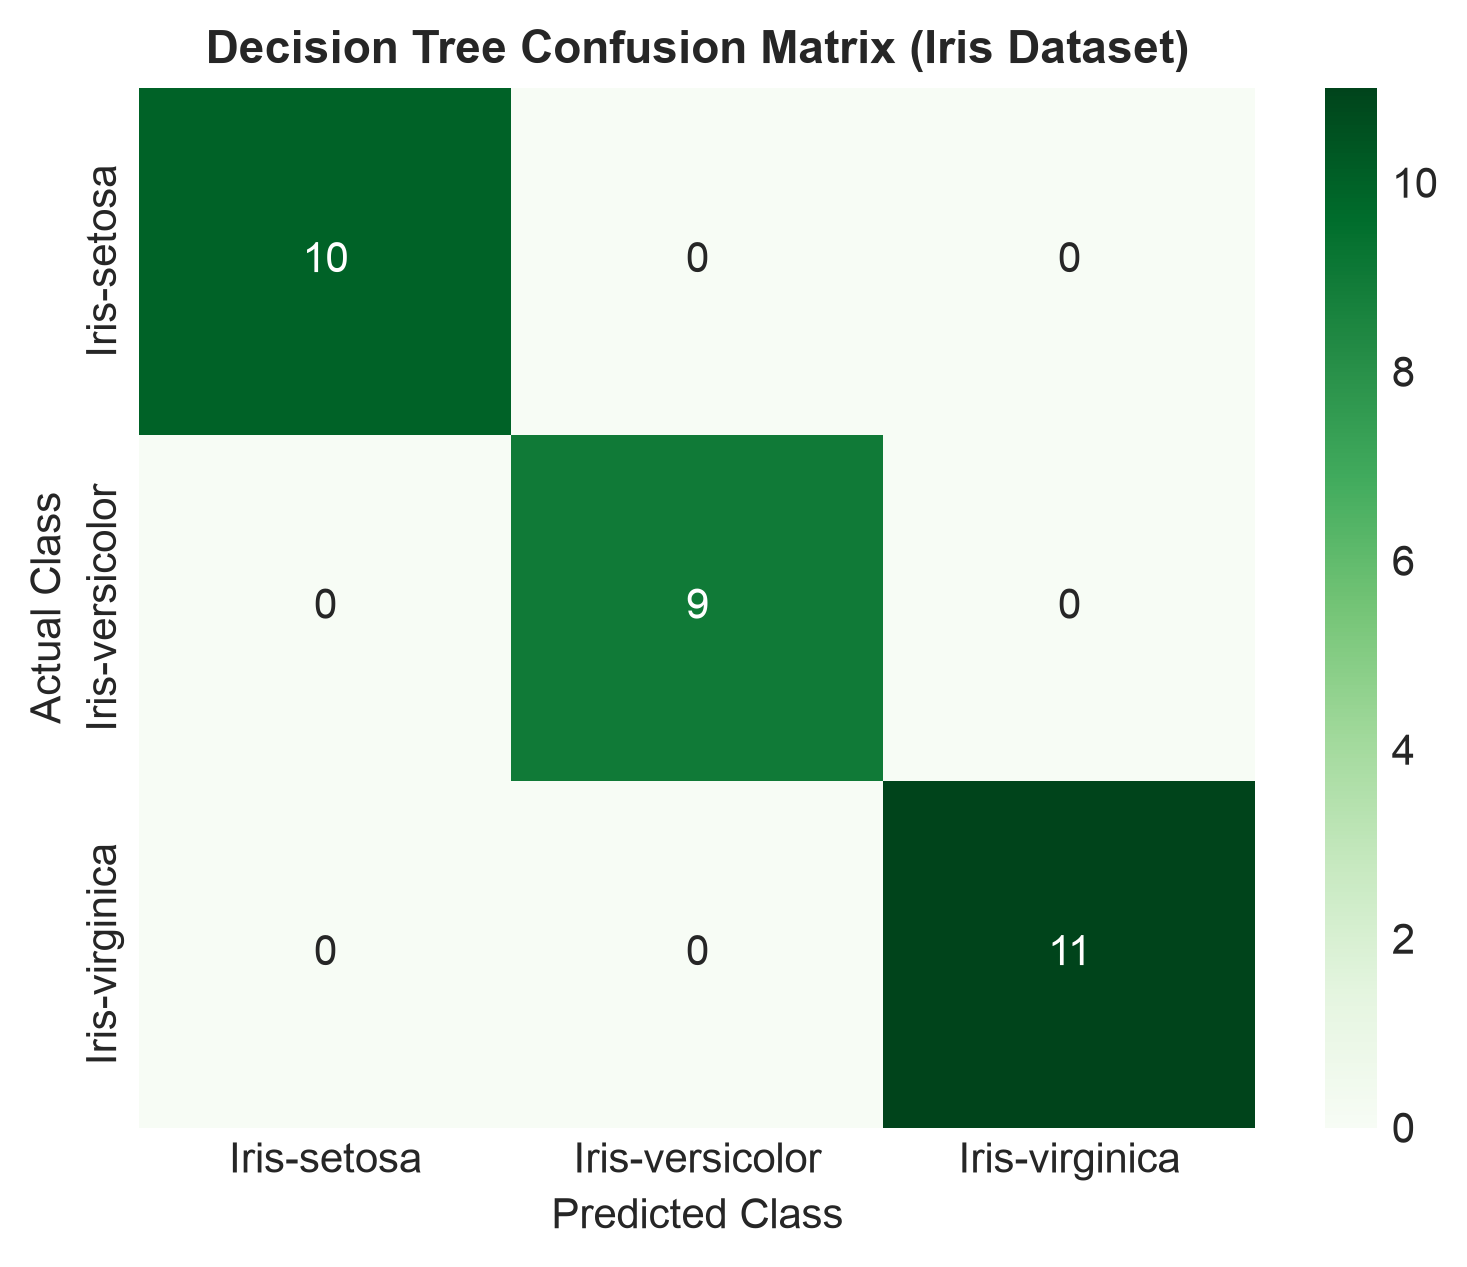
\includegraphics[width=0.55\linewidth]{images/iris_confusion_matrix.png}
\caption{Decision Tree Confusion Matrix on Iris Test Set}
\label{fig:iris_cm}
\end{figure}

\textbf{Inference:}
The confusion matrix shows zero classification errors: 10 setosa, 9 versicolor, and 11 virginica test samples were correctly predicted.

\section{Case Study 2: Loan Amount Prediction}

\subsection{Dataset Description \& ML Task}
The Loan Amount Prediction dataset contains applicant demographic details, employment status, credit history, and requested financial amounts. The target variable \texttt{LoanAmount} is continuous, formulating a \textbf{Regression} task.

\subsection{Dataset Characteristics \& Summary Statistics}
\begin{itemize}
    \item \textbf{Sample Count:} 614 initial rows. Dropped 22 rows missing \texttt{LoanAmount}, yielding 592 clean records.
    \item \textbf{Features:} 12 predictor features (4 numerical, 7 categorical, 1 identifier dropped).
    \item \textbf{Missing Values Imputed:} \texttt{Gender} (13), \texttt{Married} (3), \texttt{Dependents} (15), \texttt{Self\_Employed} (32), \texttt{Loan\_Amount\_Term} (14), \texttt{Credit\_History} (50).
    \item \textbf{Summary Statistics:} \texttt{ApplicantIncome} (Mean: \$5,405.54, Max: \$81,000), \texttt{CoapplicantIncome} (Mean: \$1,621.27), \texttt{LoanAmount} (Mean: \$146.41k, Median: \$128.00k).
\end{itemize}

\subsection{Exploratory Data Analysis}

\begin{figure}[H]
\centering
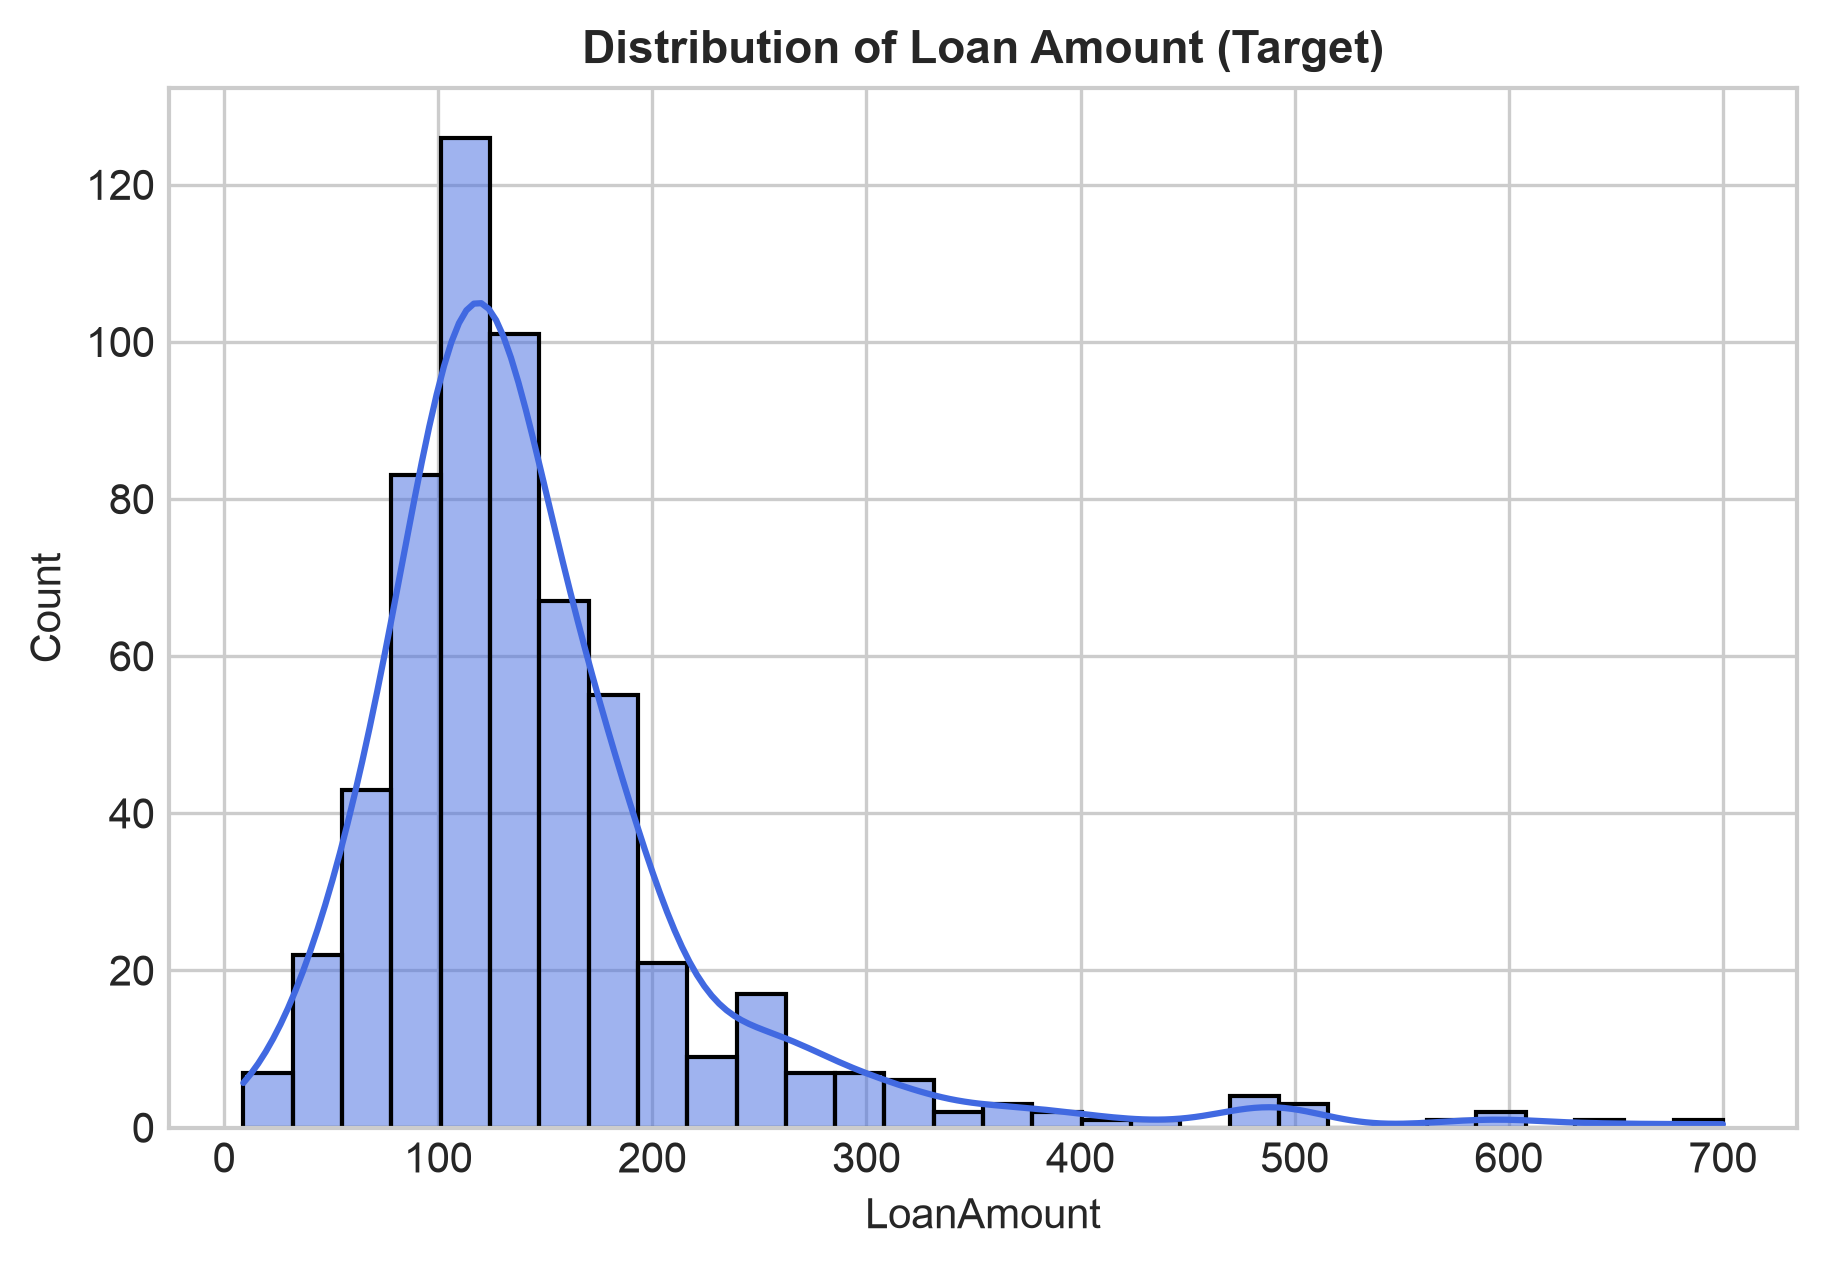
\includegraphics[width=0.7\linewidth]{images/loan_target_distribution.png}
\caption{Distribution of Loan Amount (Target Variable)}
\label{fig:loan_dist}
\end{figure}

\textbf{Inference:}
The target \texttt{LoanAmount} displays a right-skewed log-normal distribution with long upper tails, justifying natural log transformation ($\ln(1+y)$) to stabilize variance.

\begin{figure}[H]
\centering
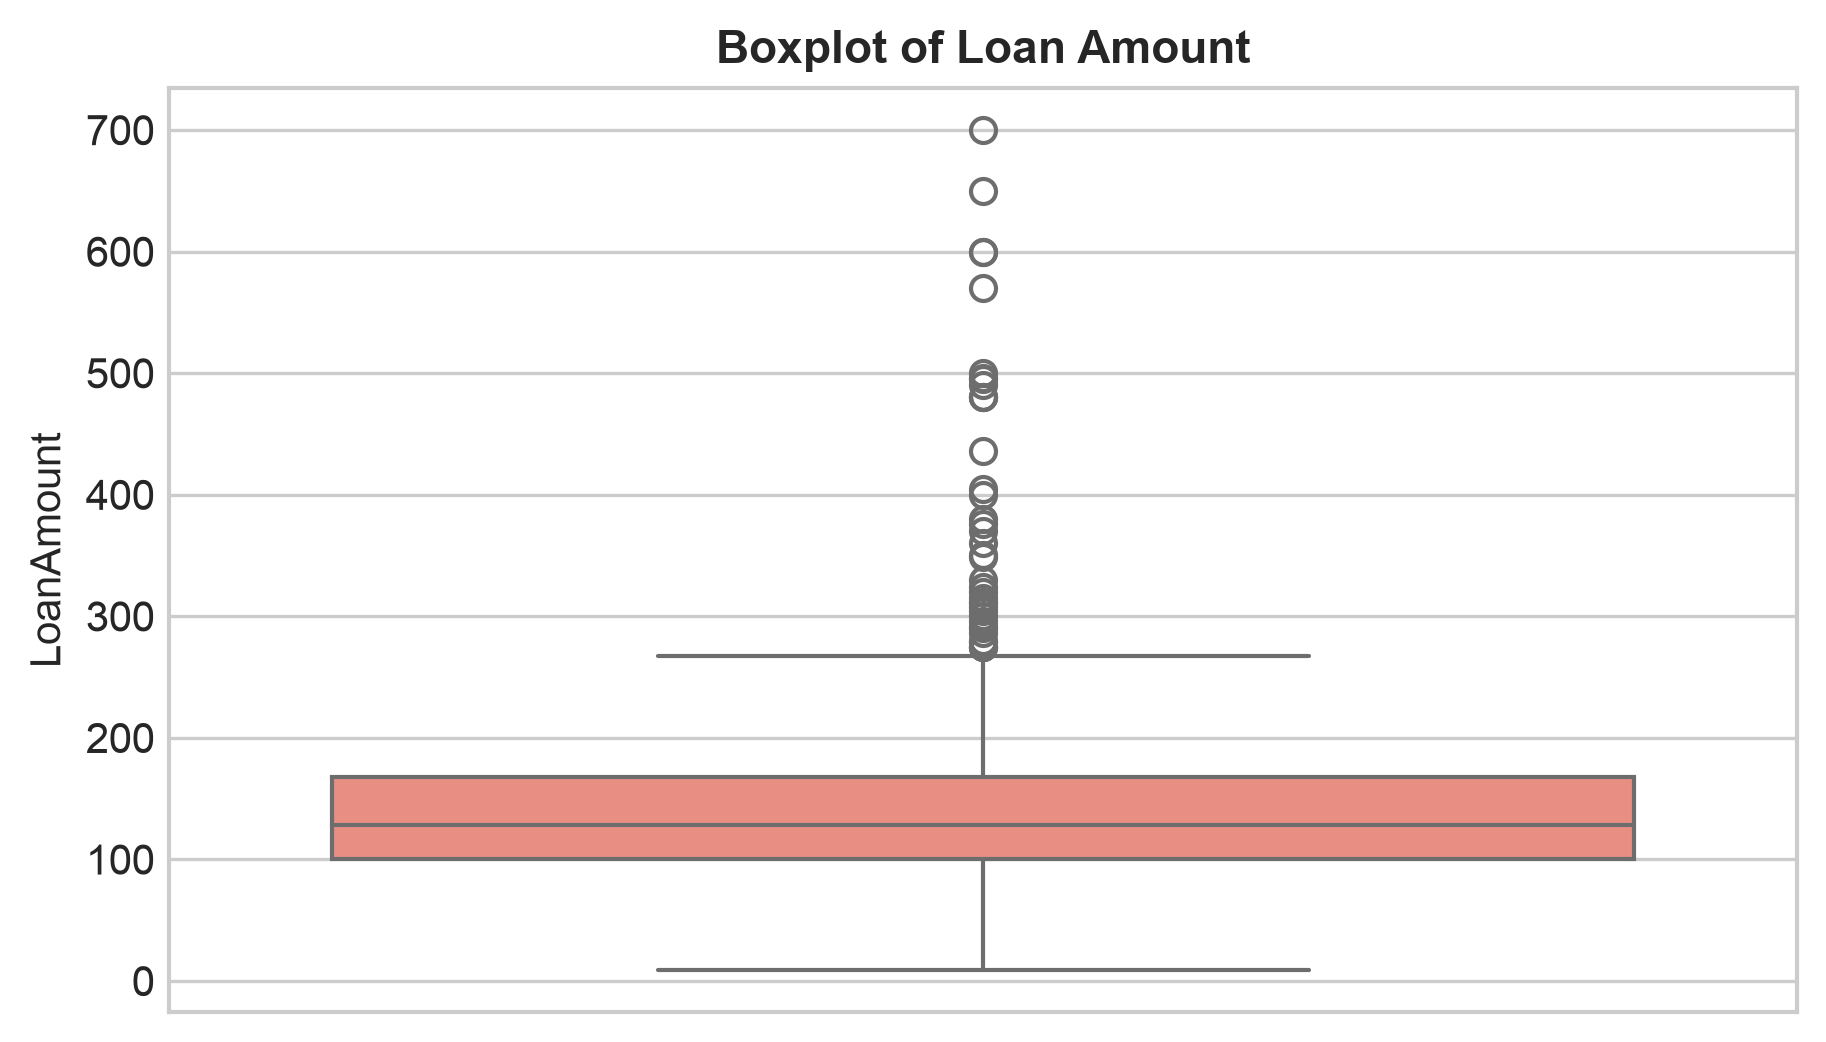
\includegraphics[width=0.65\linewidth]{images/loan_box_plot.png}
\caption{Boxplot of Loan Amount for Outlier Detection}
\label{fig:loan_box}
\end{figure}

\textbf{Inference:}
Numerous extreme upper outliers exist above \$300,000, confirming that applicant requests span diverse credit brackets.

\begin{figure}[H]
\centering
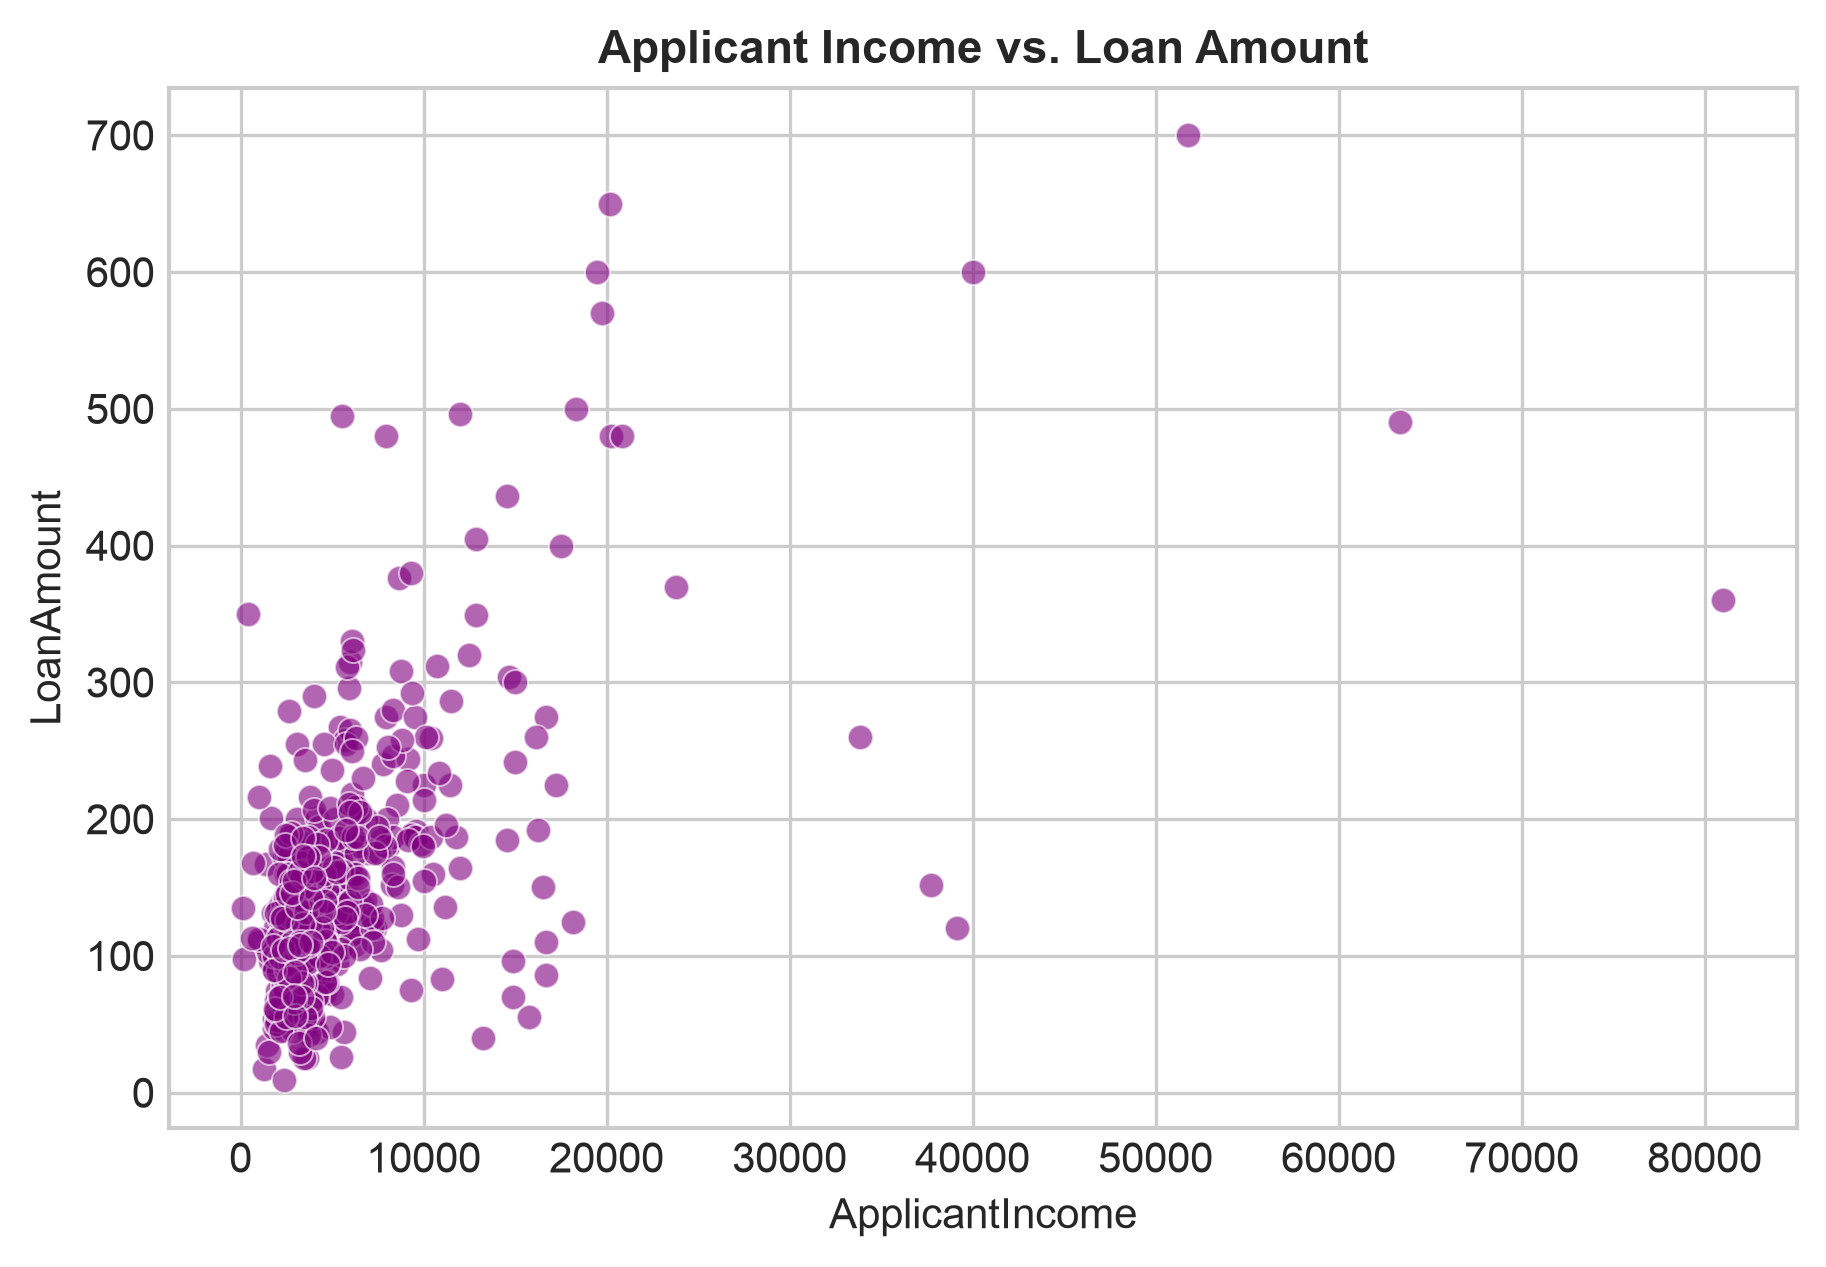
\includegraphics[width=0.7\linewidth]{images/loan_income_vs_amount.png}
\caption{Applicant Income vs. Loan Amount Scatter Plot}
\label{fig:loan_scatter}
\end{figure}

\textbf{Inference:}
A positive linear relation is present between income and loan size, with variance expanding at higher income levels.

\begin{figure}[H]
\centering
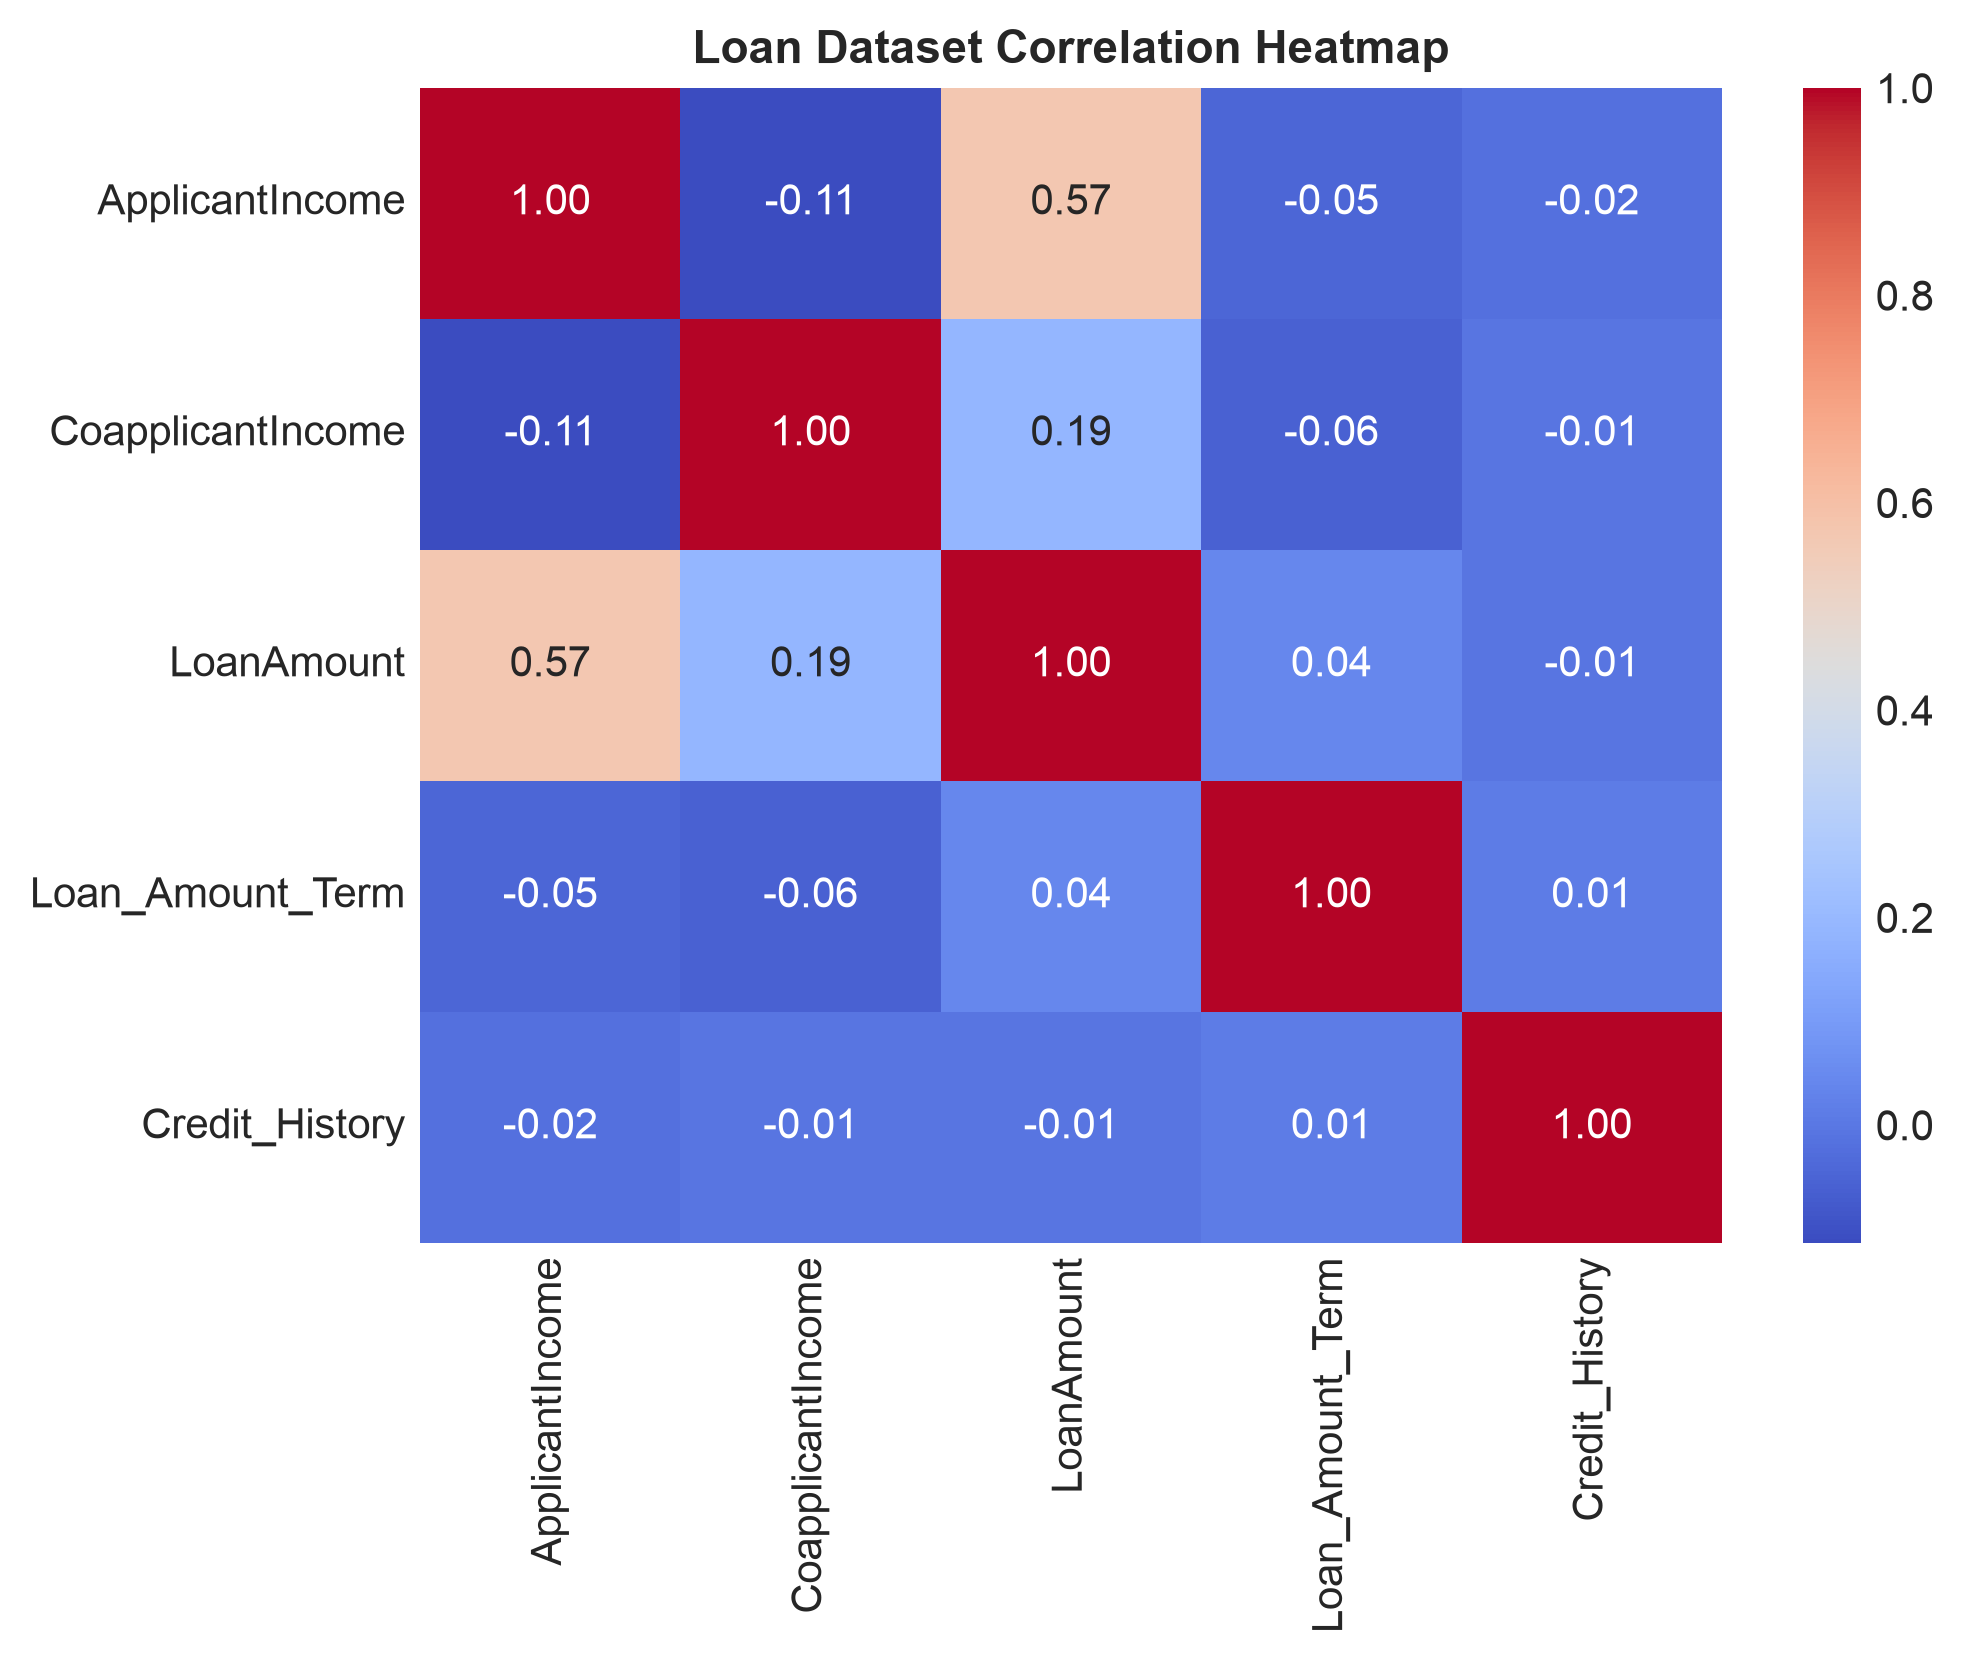
\includegraphics[width=0.65\linewidth]{images/loan_correlation_heatmap.png}
\caption{Correlation Heatmap of Numerical Features}
\label{fig:loan_corr}
\end{figure}

\textbf{Inference:}
\texttt{ApplicantIncome} correlates positively with \texttt{LoanAmount} ($r = 0.57$).

\subsection{Data Preprocessing \& Model Evaluation}
\begin{itemize}
    \item \textbf{Preprocessing:} Categorical missing values imputed with column mode; numerical missing values imputed with column median. One-Hot Encoding applied to categorical variables (\texttt{drop\_first=True}). Target transformed via \texttt{np.log1p(LoanAmount)}.
    \item \textbf{Model Trained:} \texttt{RandomForestRegressor(n\_estimators=200, random\_state=42)}.
    \item \textbf{Regression Performance Metrics:}
    \begin{itemize}
        \item Mean Absolute Error (MAE): \textbf{0.2529}
        \item Root Mean Squared Error (RMSE): \textbf{0.3604}
        \item $R^2$ Score: \textbf{0.3228}
    \end{itemize}
\end{itemize}

\section{Case Study 3: Classification of Email Spam}

\subsection{Dataset Description \& ML Task}
The SMS Spam Collection dataset contains text messages tagged as \texttt{ham} (legitimate) or \texttt{spam}. The objective is a \textbf{Binary Text Classification} task using Natural Language Processing (NLP).

\subsection{Dataset Characteristics \& Summary Statistics}
\begin{itemize}
    \item \textbf{Total Instances:} 5,572 text messages.
    \item \textbf{Class Distribution:} 4,825 \texttt{ham} (86.6\%) vs. 747 \texttt{spam} (13.4\%) instances.
    \item \textbf{Message Length Stats:} Ham length (Mean: 71.0 characters, Median: 52.0), Spam length (Mean: 138.9 characters, Median: 149.0).
\end{itemize}

\subsection{Exploratory Data Analysis}

\begin{figure}[H]
\centering
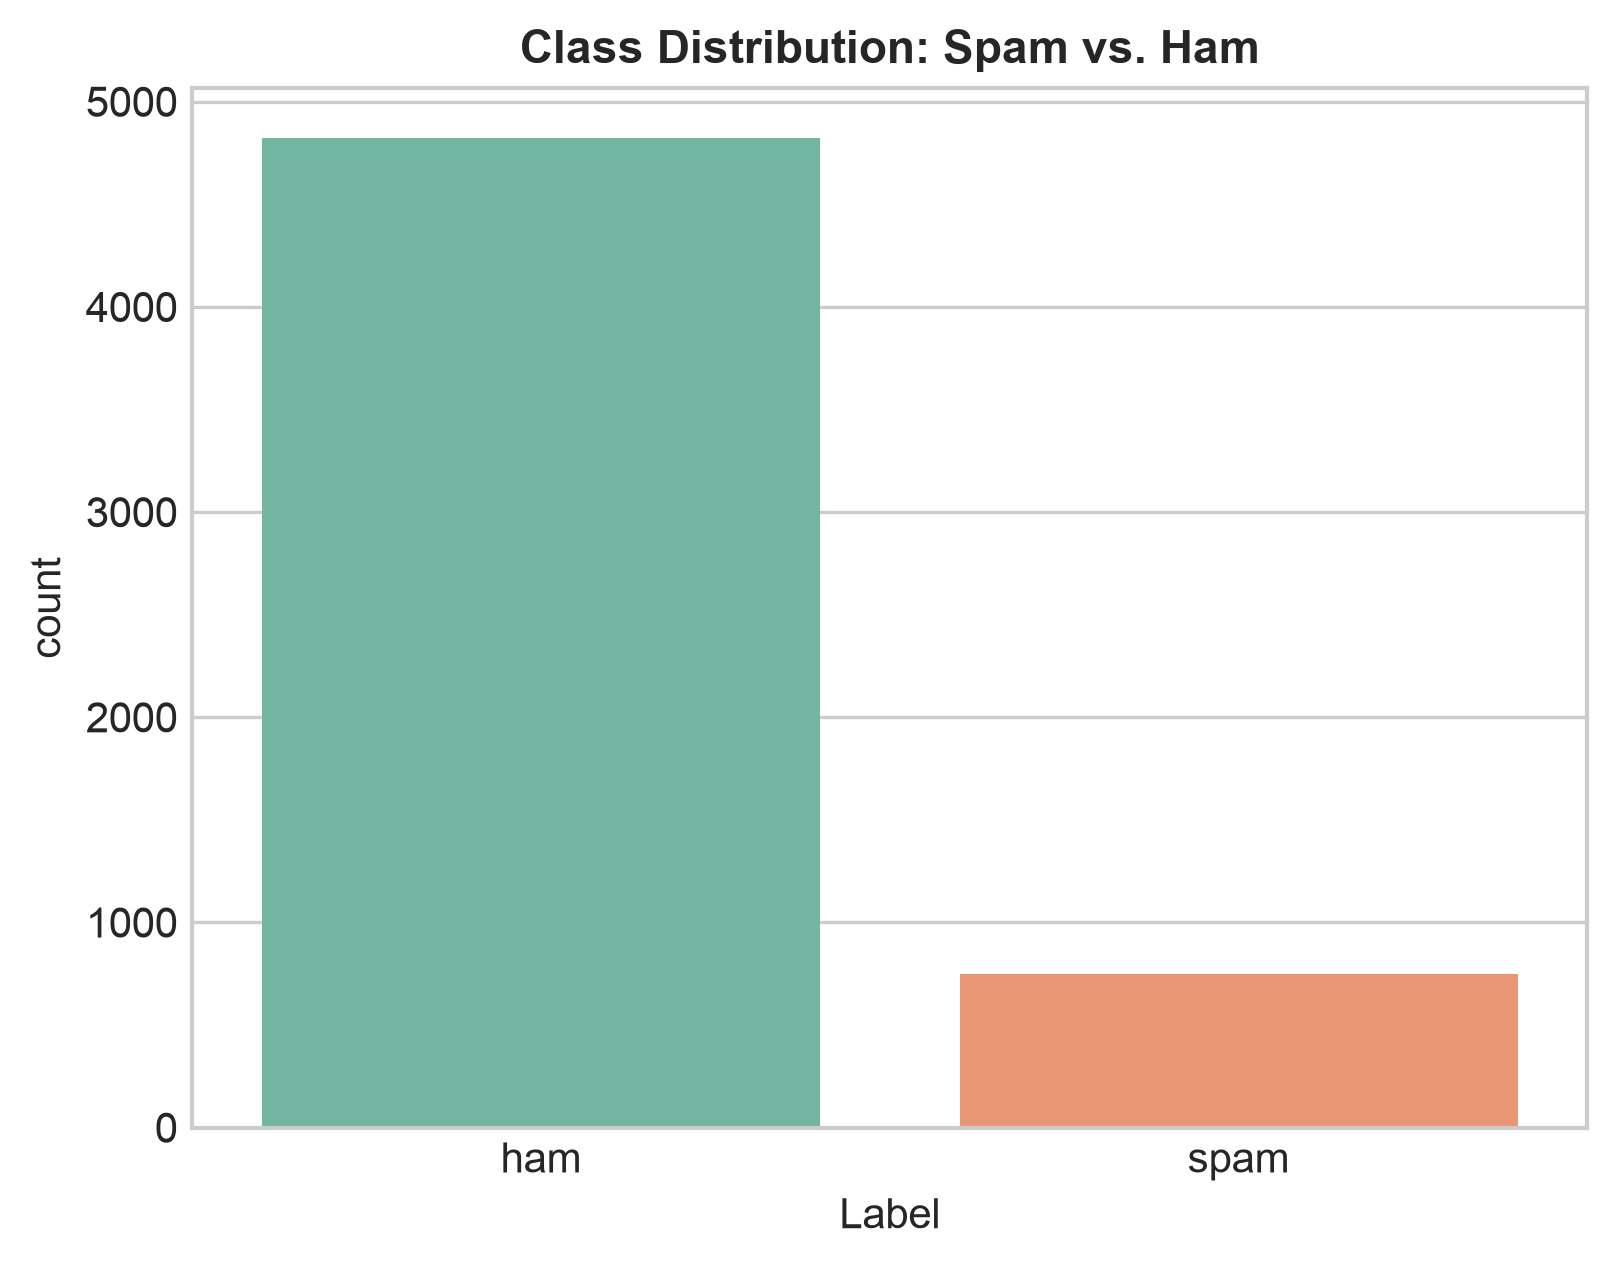
\includegraphics[width=0.6\linewidth]{images/spam_count.png}
\caption{Class Countplot: Spam vs. Ham Messages}
\label{fig:spam_count}
\end{figure}

\textbf{Inference:}
The dataset exhibits severe class imbalance, with legitimate messages outnumbering spam messages by more than 6:1.

\begin{figure}[H]
\centering
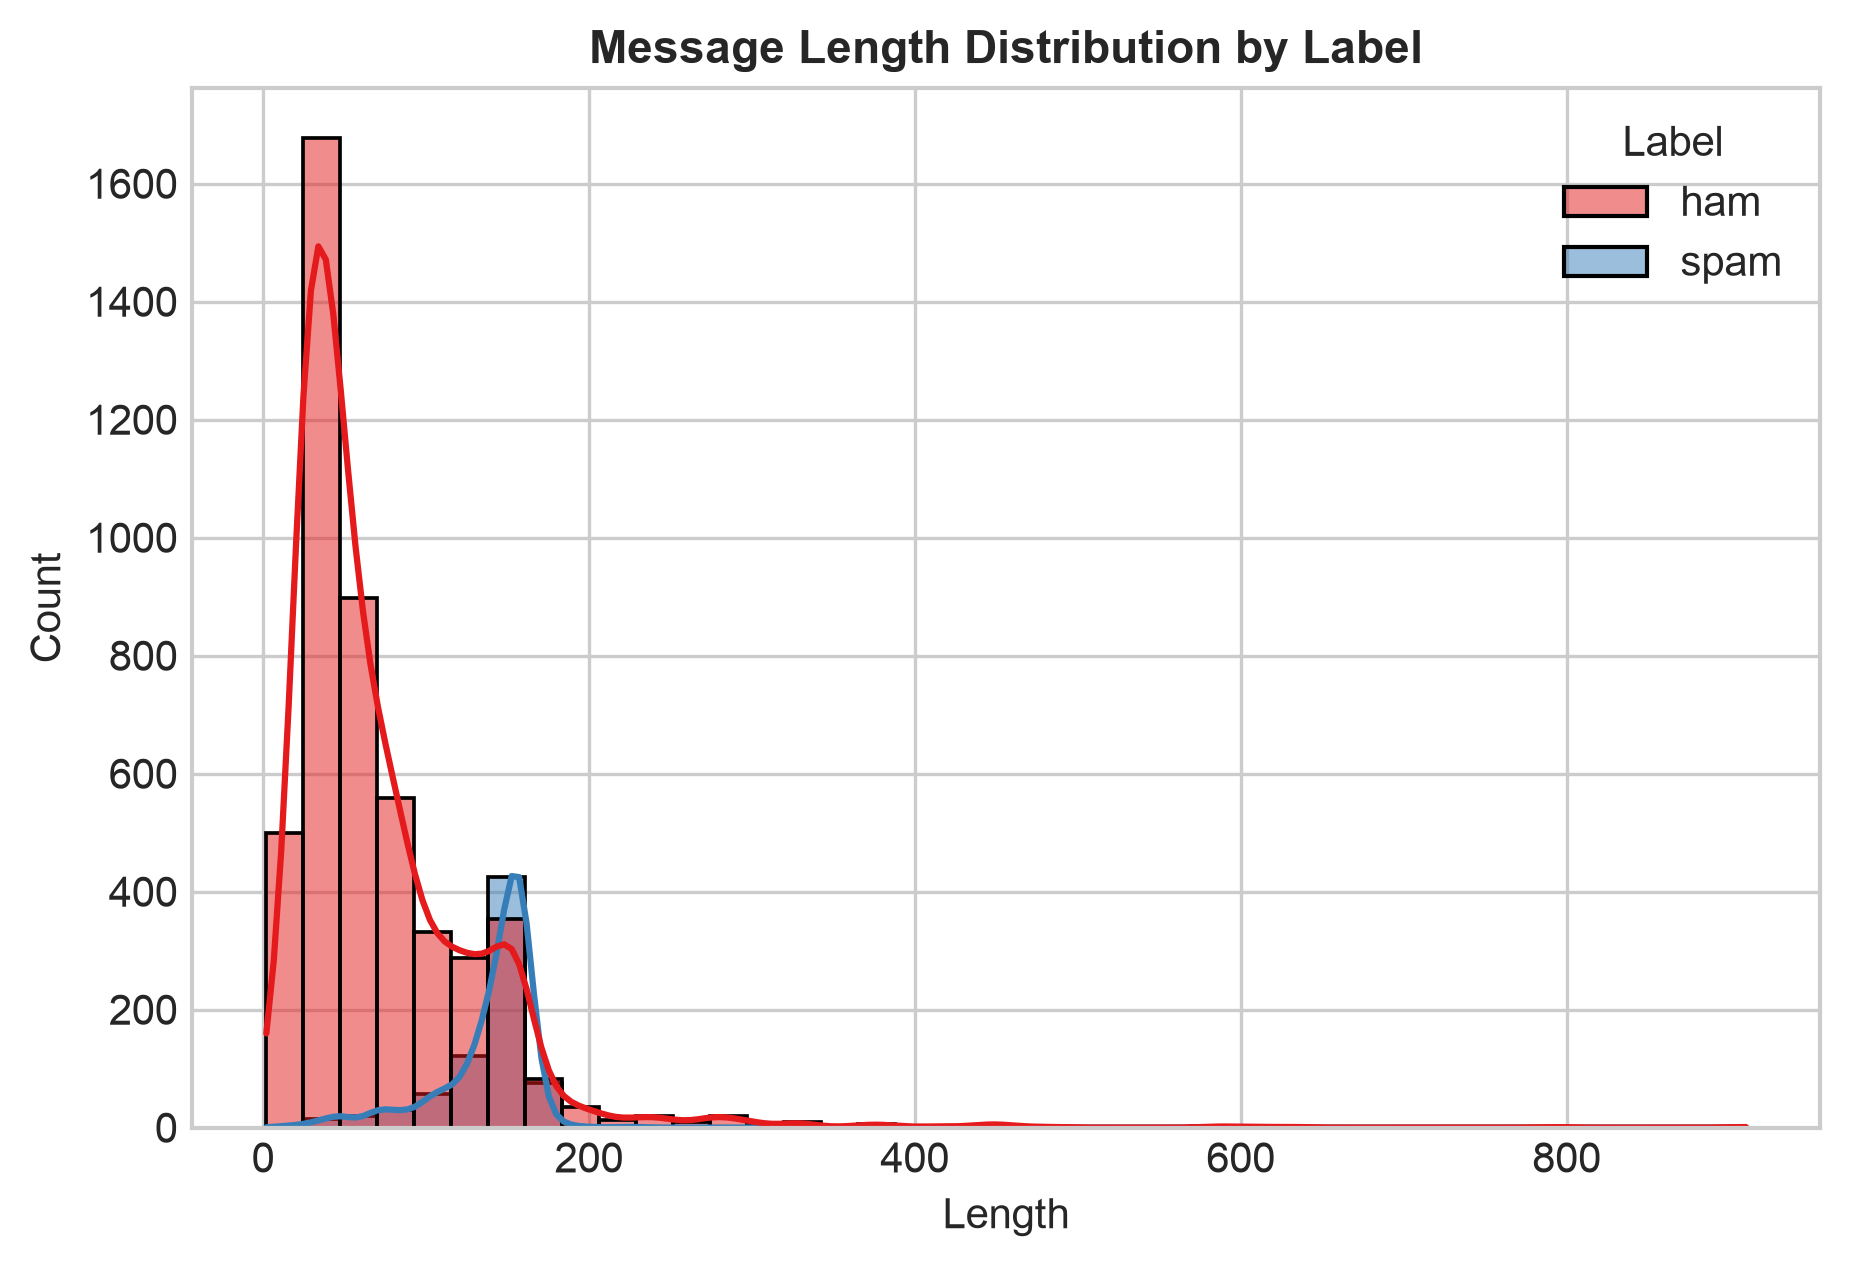
\includegraphics[width=0.75\linewidth]{images/spam_length_distribution.png}
\caption{Histogram of Message Character Length by Label}
\label{fig:spam_dist}
\end{figure}

\textbf{Inference:}
Spam messages cluster heavily around 130--160 characters (nearing SMS carrier limits), whereas ham messages are generally concise ($< 80$ characters).

\begin{figure}[H]
\centering
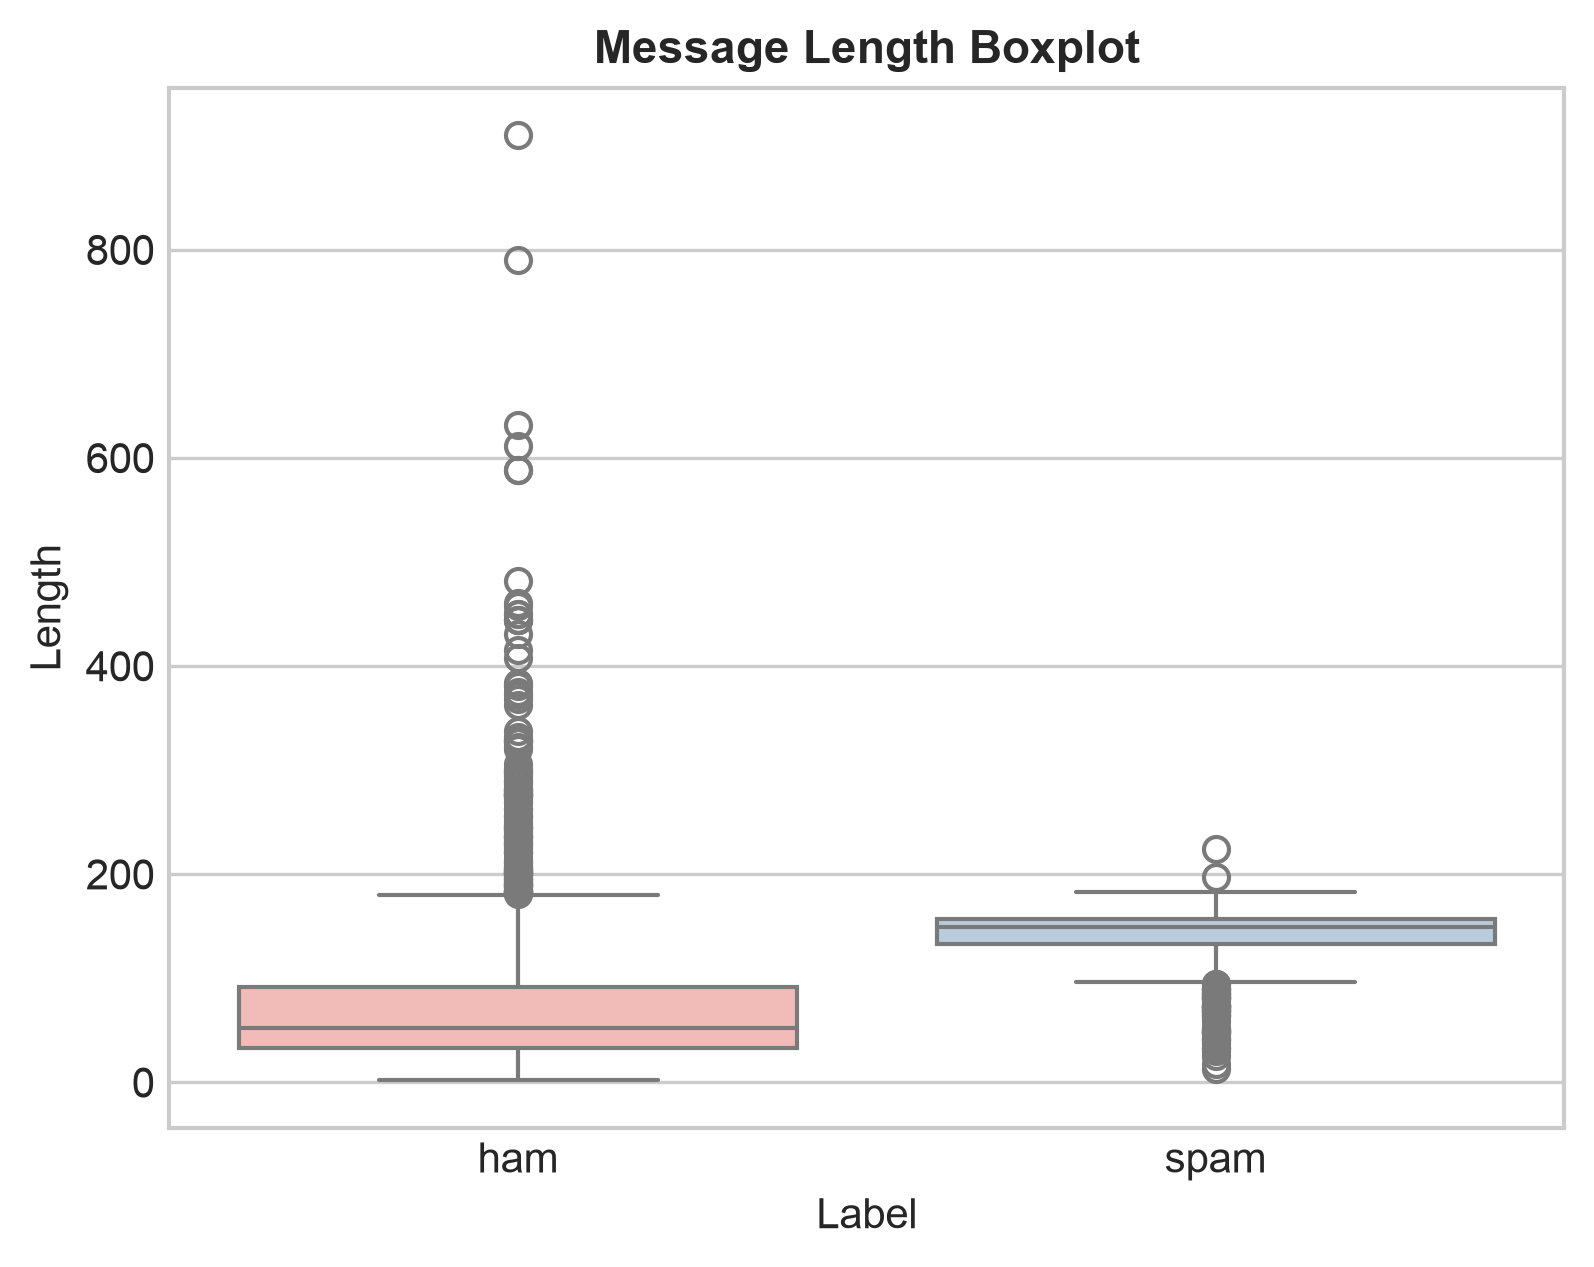
\includegraphics[width=0.6\linewidth]{images/spam_length_boxplot.png}
\caption{Boxplot of Message Length across Classes}
\label{fig:spam_box}
\end{figure}

\textbf{Inference:}
Boxplots confirm that message length provides strong linear discriminative power between spam and ham messages.

\begin{figure}[H]
\centering
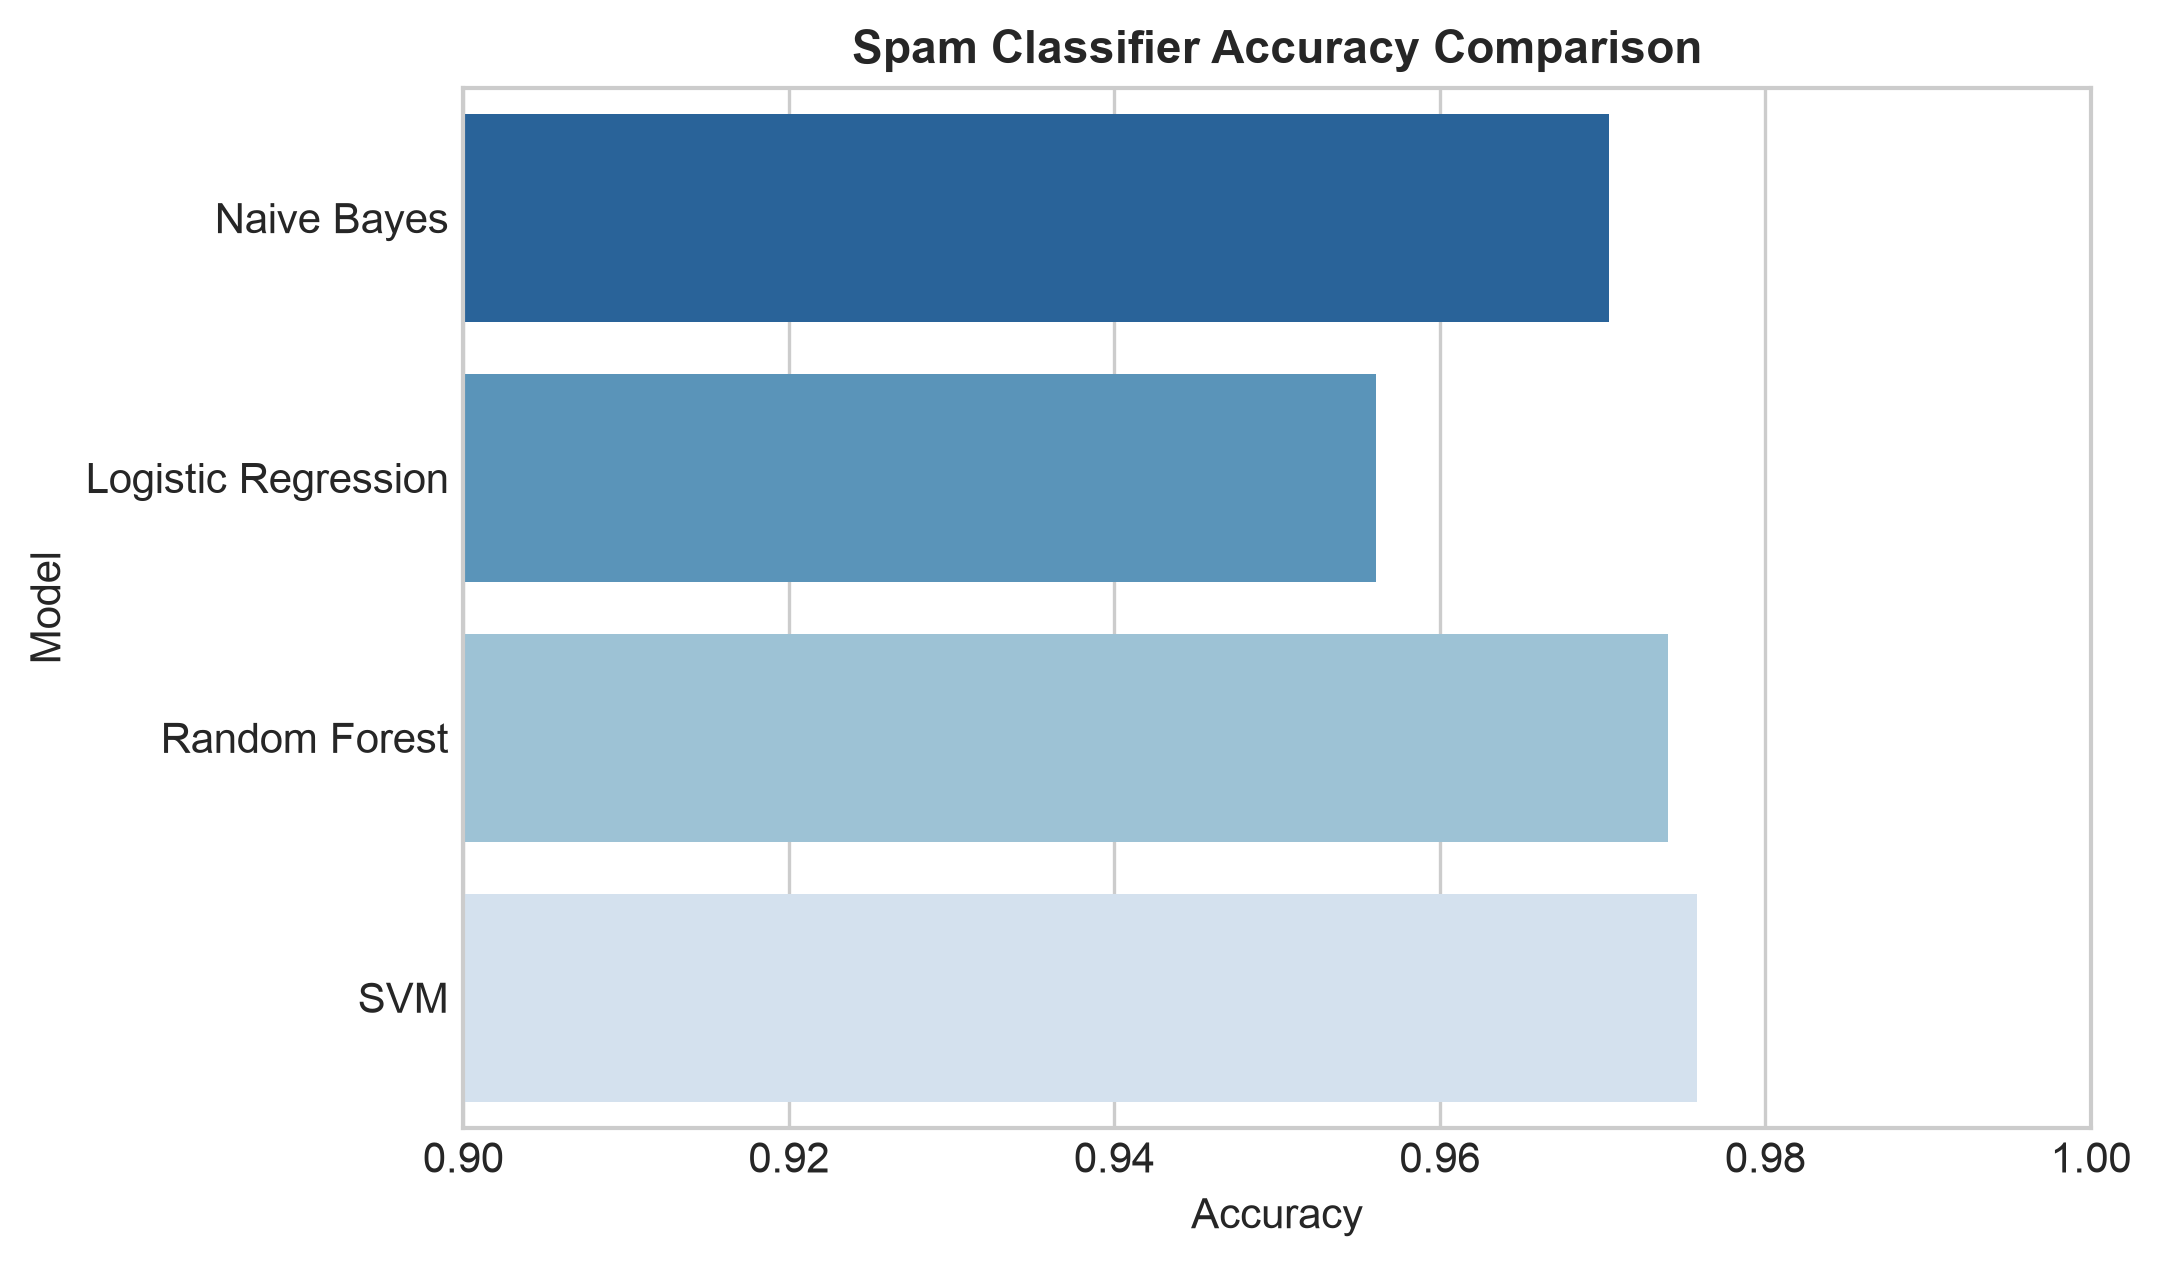
\includegraphics[width=0.7\linewidth]{images/spam_models_comparison.png}
\caption{Accuracy Comparison of Text Classification Models}
\label{fig:spam_comp}
\end{figure}

\textbf{Inference:}
Support Vector Machines (SVM) achieved the highest overall accuracy of \textbf{97.58\%}, slightly outperforming Random Forest (97.40\%) and Naive Bayes (97.04\%).

\subsection{Data Preprocessing \& Model Evaluation}
\begin{itemize}
    \item \textbf{Feature Extraction:} Converted raw text into TF-IDF numerical matrices (\texttt{TfidfVectorizer(max\_features=3000)}).
    \item \textbf{Model Performance Summary:}
    \begin{itemize}
        \item Multinomial Naive Bayes: Accuracy = \textbf{0.9704}
        \item Logistic Regression: Accuracy = \textbf{0.9561}
        \item Random Forest Classifier: Accuracy = \textbf{0.9740}
        \item \textbf{Support Vector Machine (SVM): Accuracy = 0.9758}
    \end{itemize}
\end{itemize}

\section{Case Study 4: Predicting Diabetes}

\subsection{Dataset Description \& ML Task}
The Pima Indians Diabetes dataset contains diagnostic medical measurements from female patients. The task is a \textbf{Binary Medical Classification} to predict whether a patient has diabetes (\texttt{Outcome = 1}).

\subsection{Dataset Characteristics \& Summary Statistics}
\begin{itemize}
    \item \textbf{Total Instances:} 768 patient records.
    \item \textbf{Class Breakdown:} 500 Non-diabetic (\texttt{Outcome = 0}) vs. 268 Diabetic (\texttt{Outcome = 1}).
    \item \textbf{Physiologically Invalid Zero Values:} \texttt{Glucose} (5 zeros), \texttt{BloodPressure} (35 zeros), \texttt{SkinThickness} (227 zeros), \texttt{Insulin} (374 zeros), \texttt{BMI} (11 zeros).
\end{itemize}

\subsection{Exploratory Data Analysis}

\begin{figure}[H]
\centering
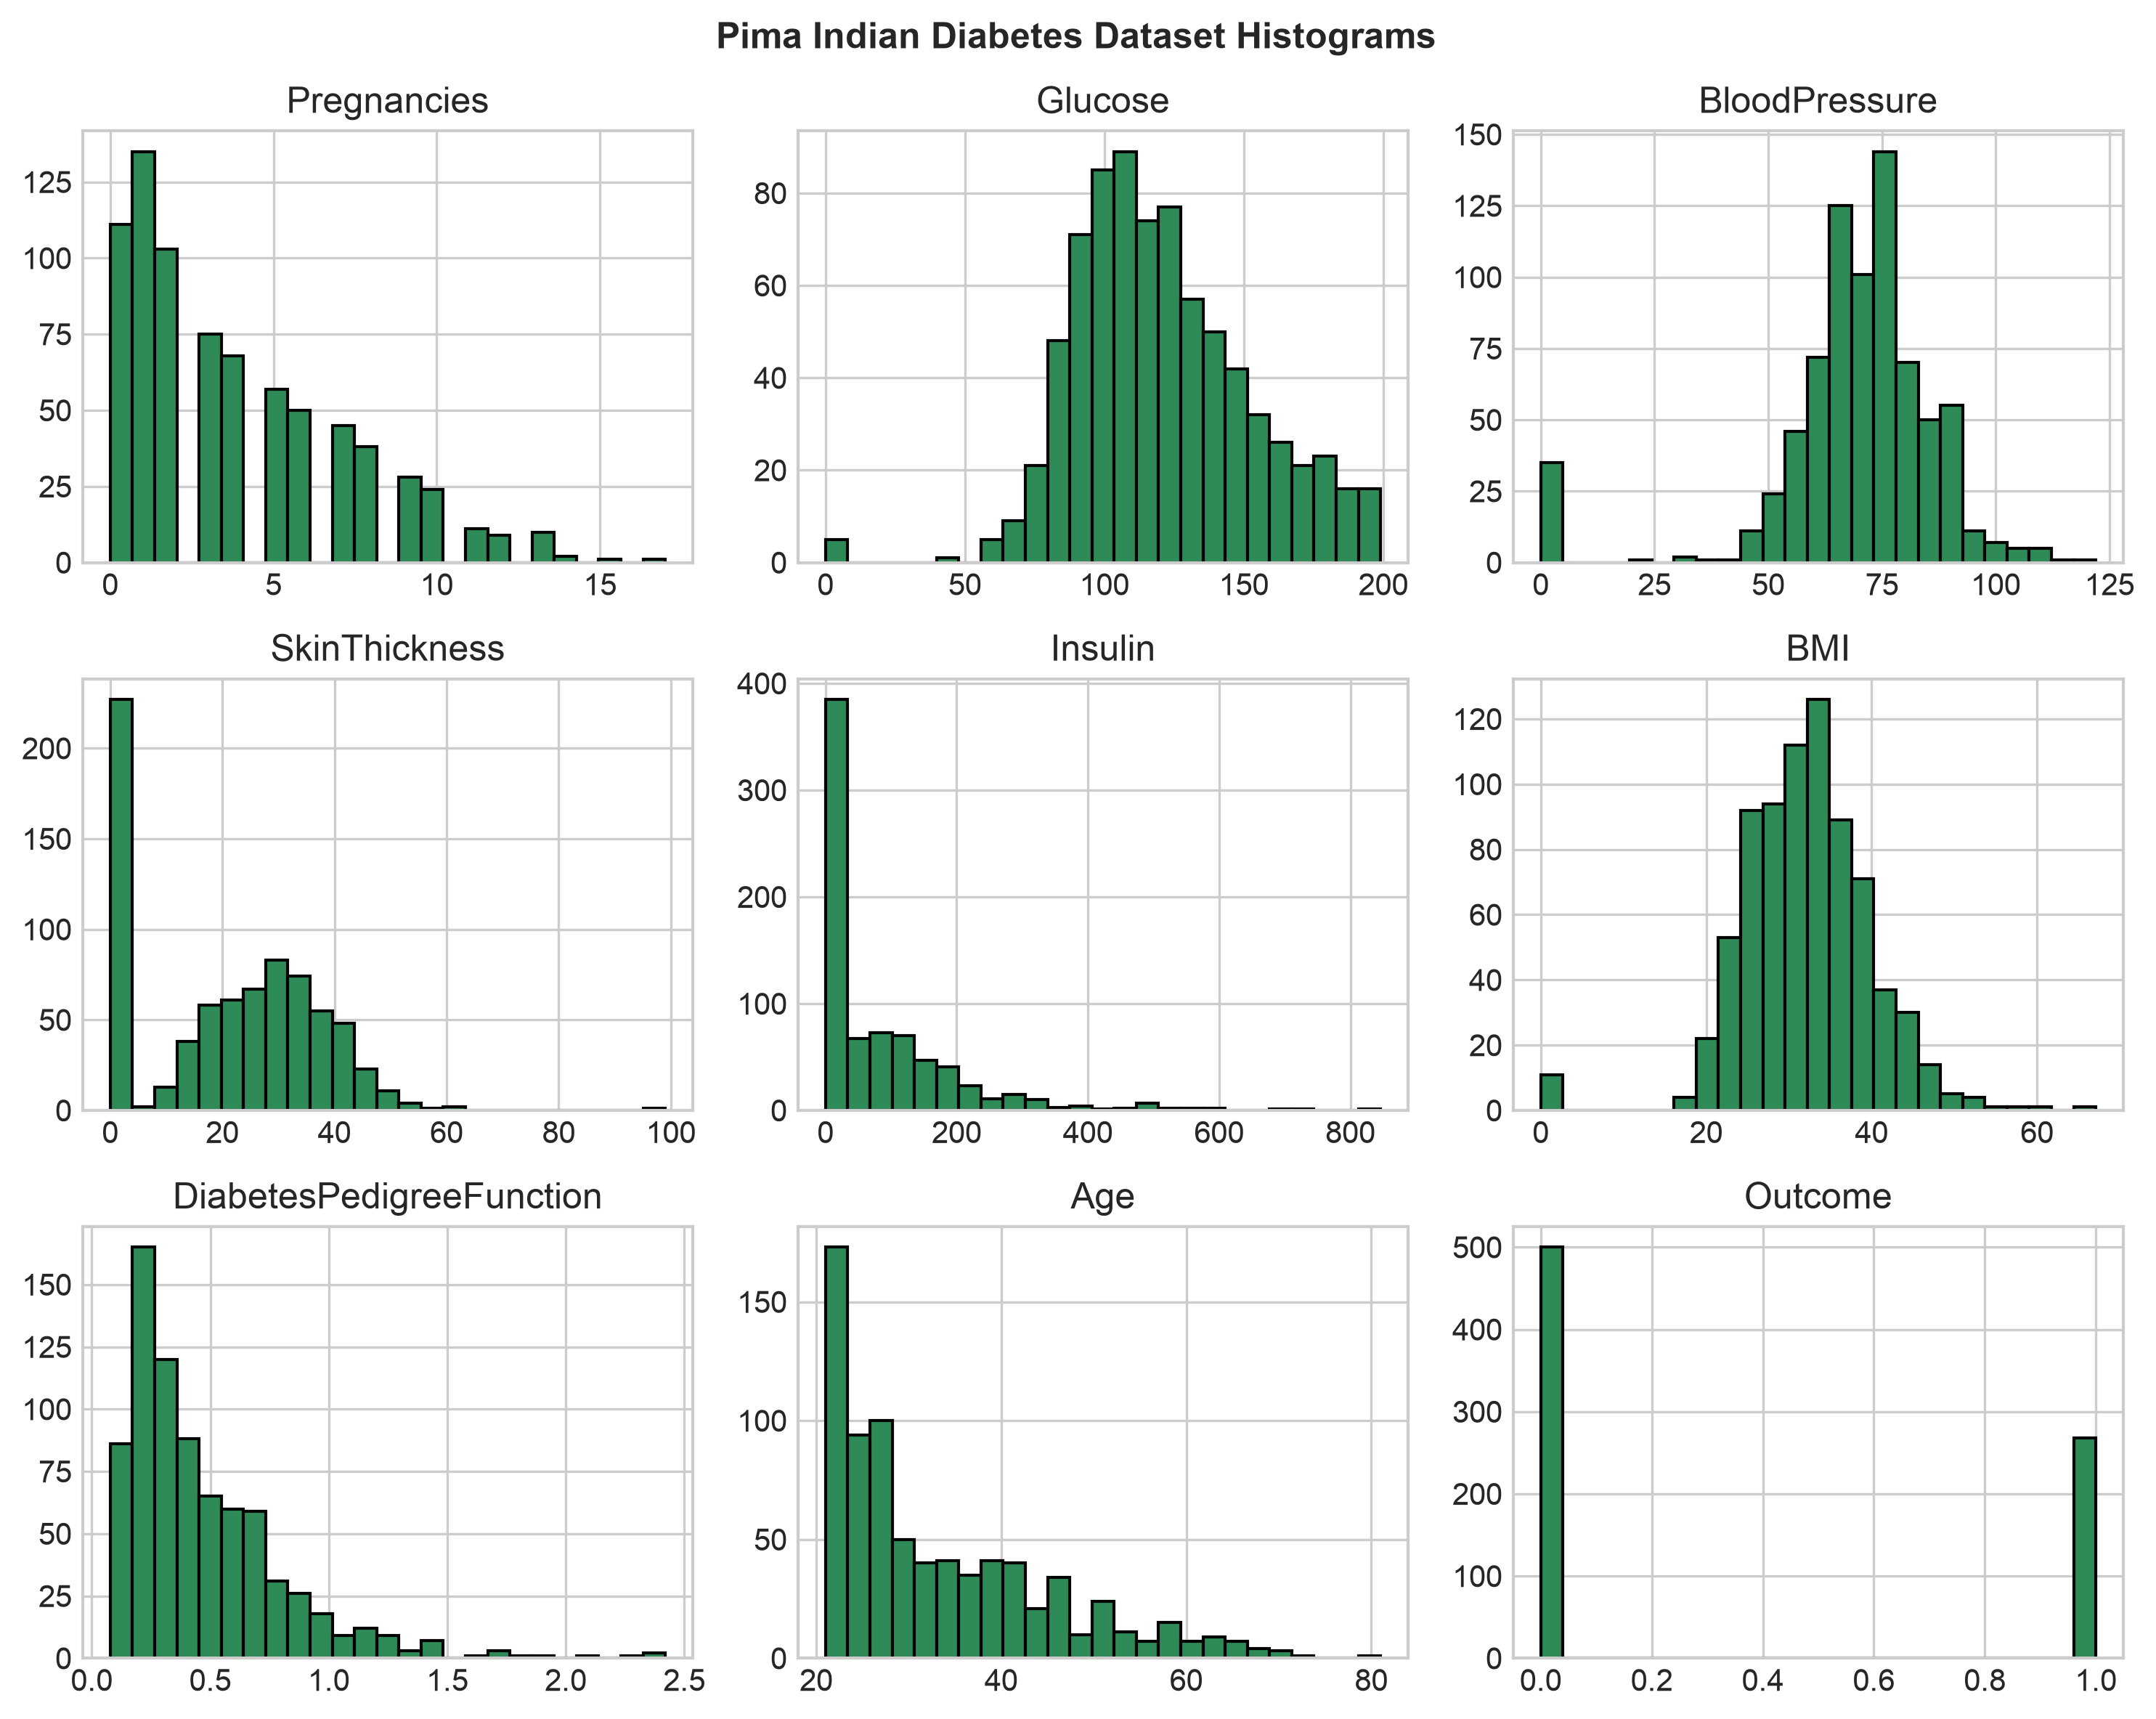
\includegraphics[width=0.8\linewidth]{images/diabetes_histograms.png}
\caption{Histograms of Diabetes Clinical Features}
\label{fig:diab_hist}
\end{figure}

\textbf{Inference:}
Features like \texttt{Insulin} and \texttt{DiabetesPedigreeFunction} exhibit sharp positive skewness, while \texttt{Glucose} follows a normal distribution centered near 120 mg/dL.

\begin{figure}[H]
\centering
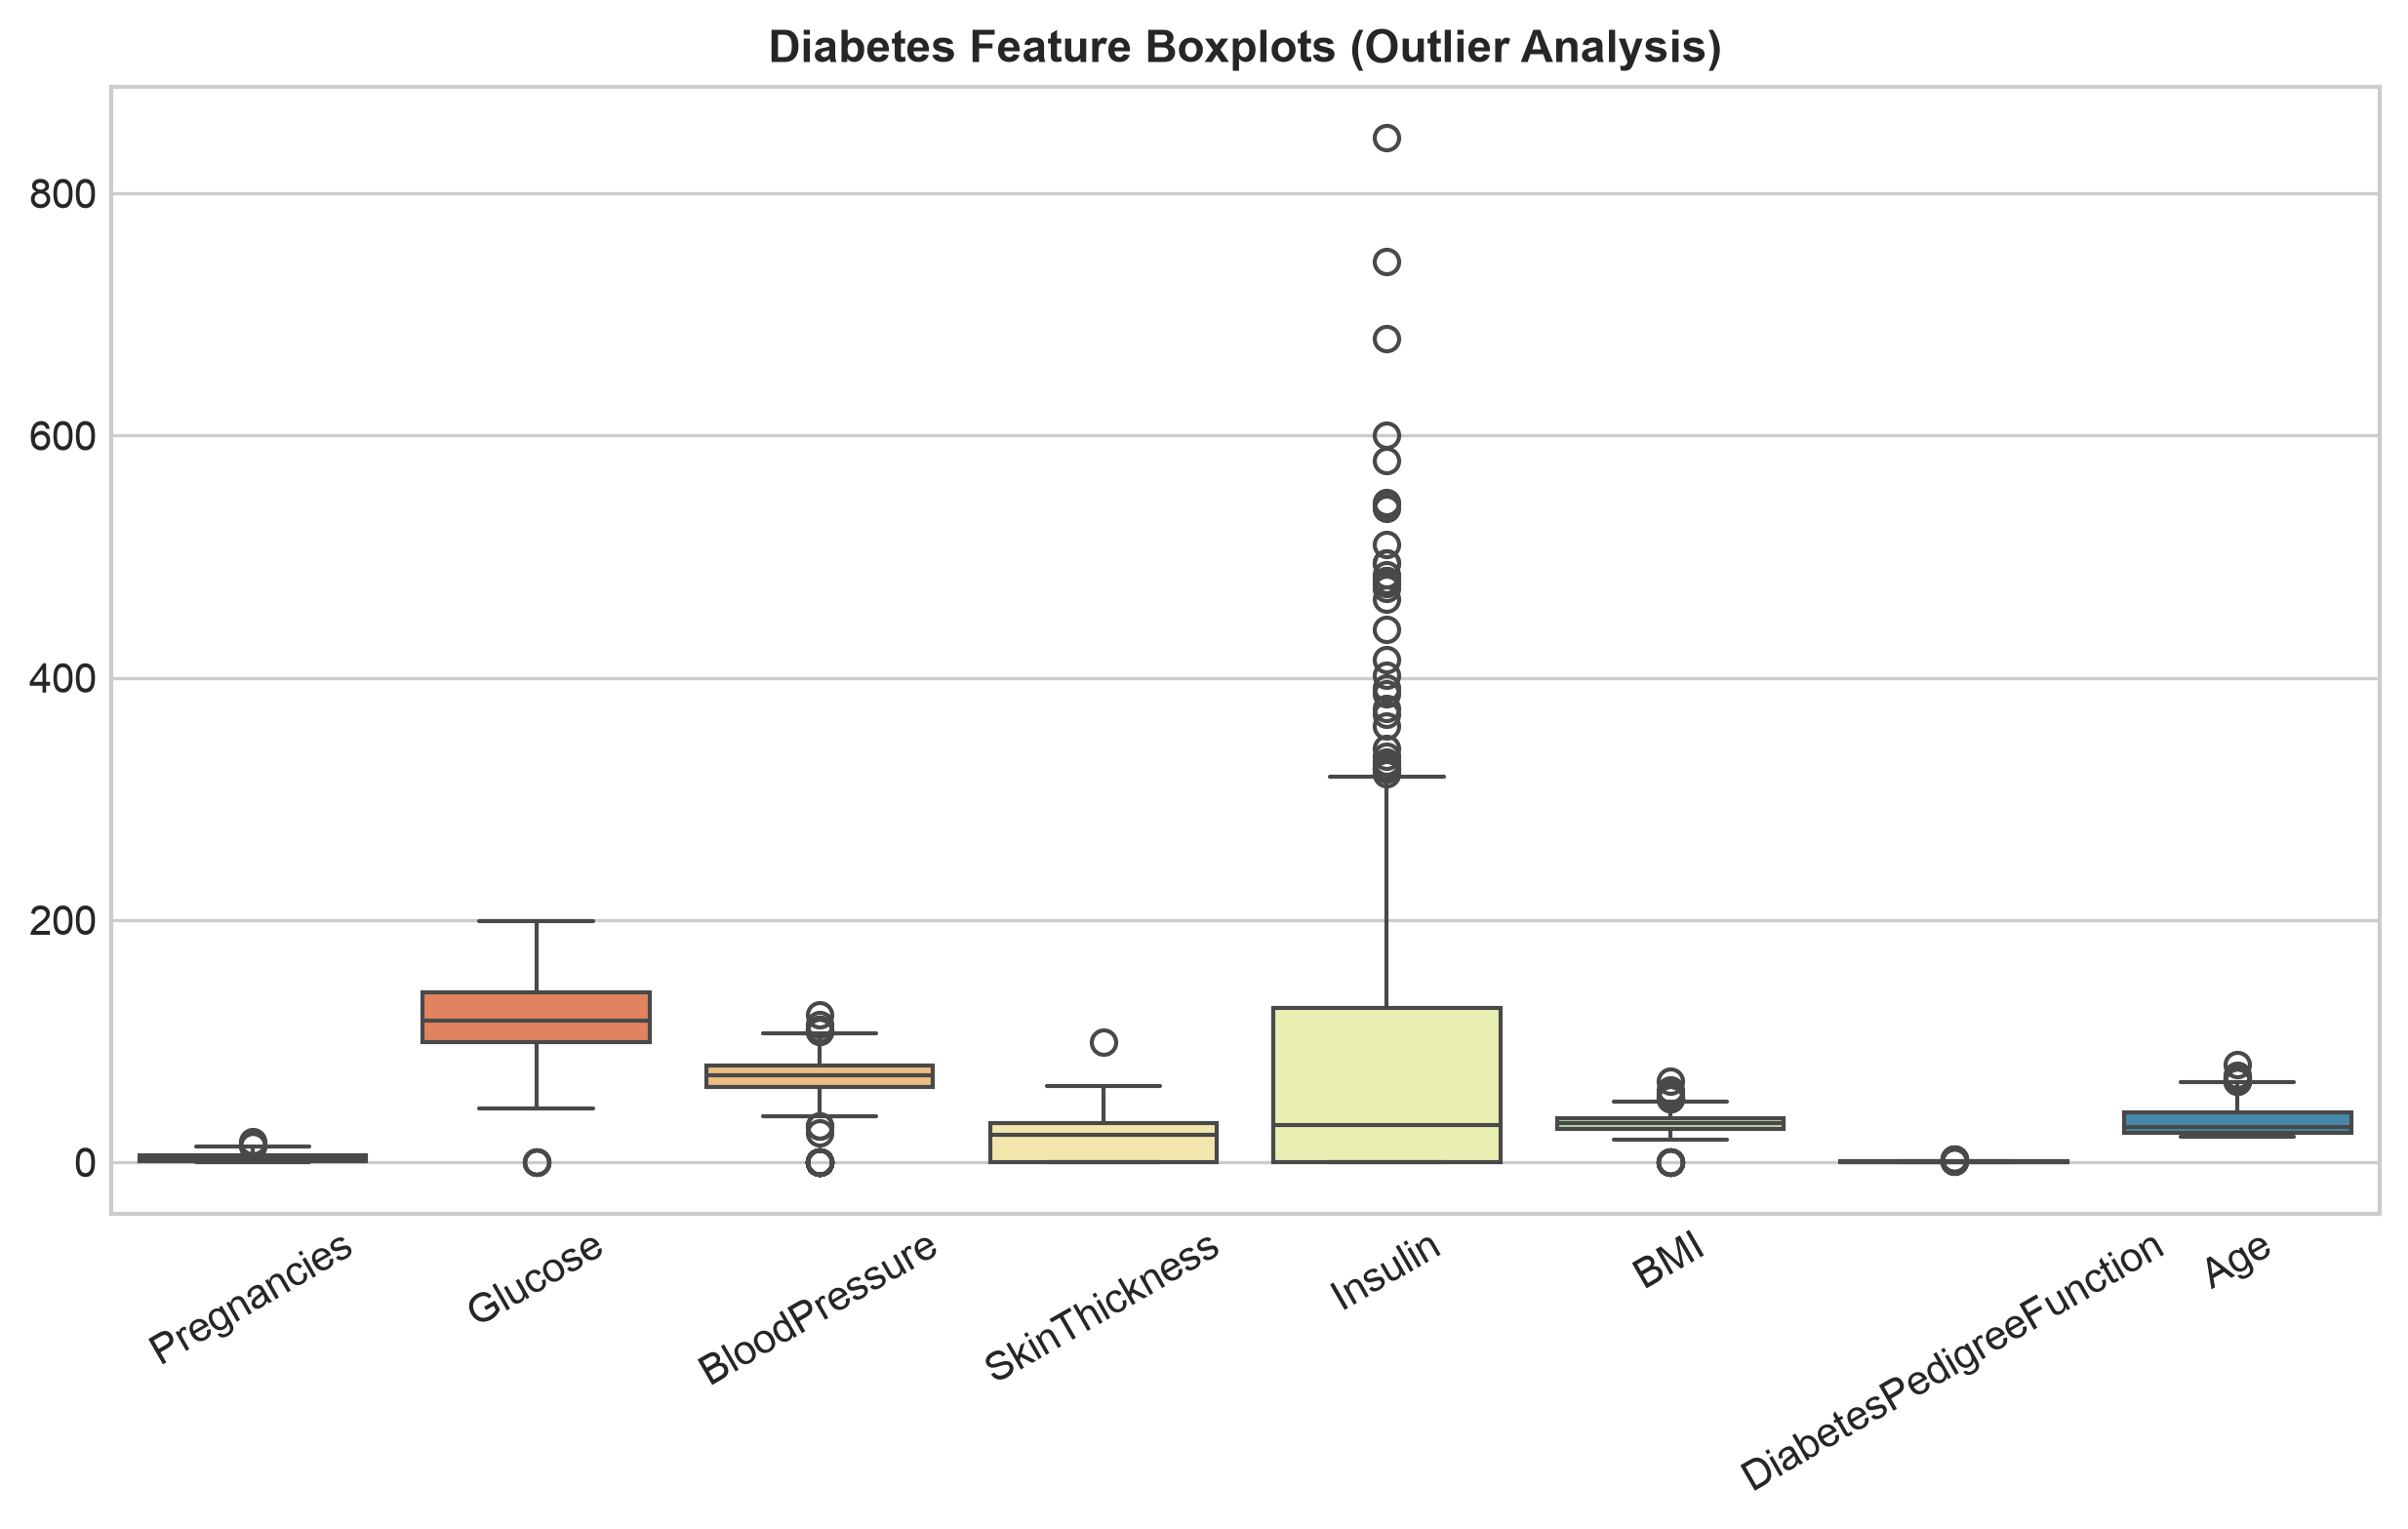
\includegraphics[width=0.8\linewidth]{images/diabetes_boxplots.png}
\caption{Boxplots of Diabetes Predictor Features}
\label{fig:diab_box}
\end{figure}

\textbf{Inference:}
Outlier analysis indicates high upper values in \texttt{Insulin} ($> 400$) and \texttt{Glucose}. Imputing zeros with column medians prevents distance distortions.

\begin{figure}[H]
\centering
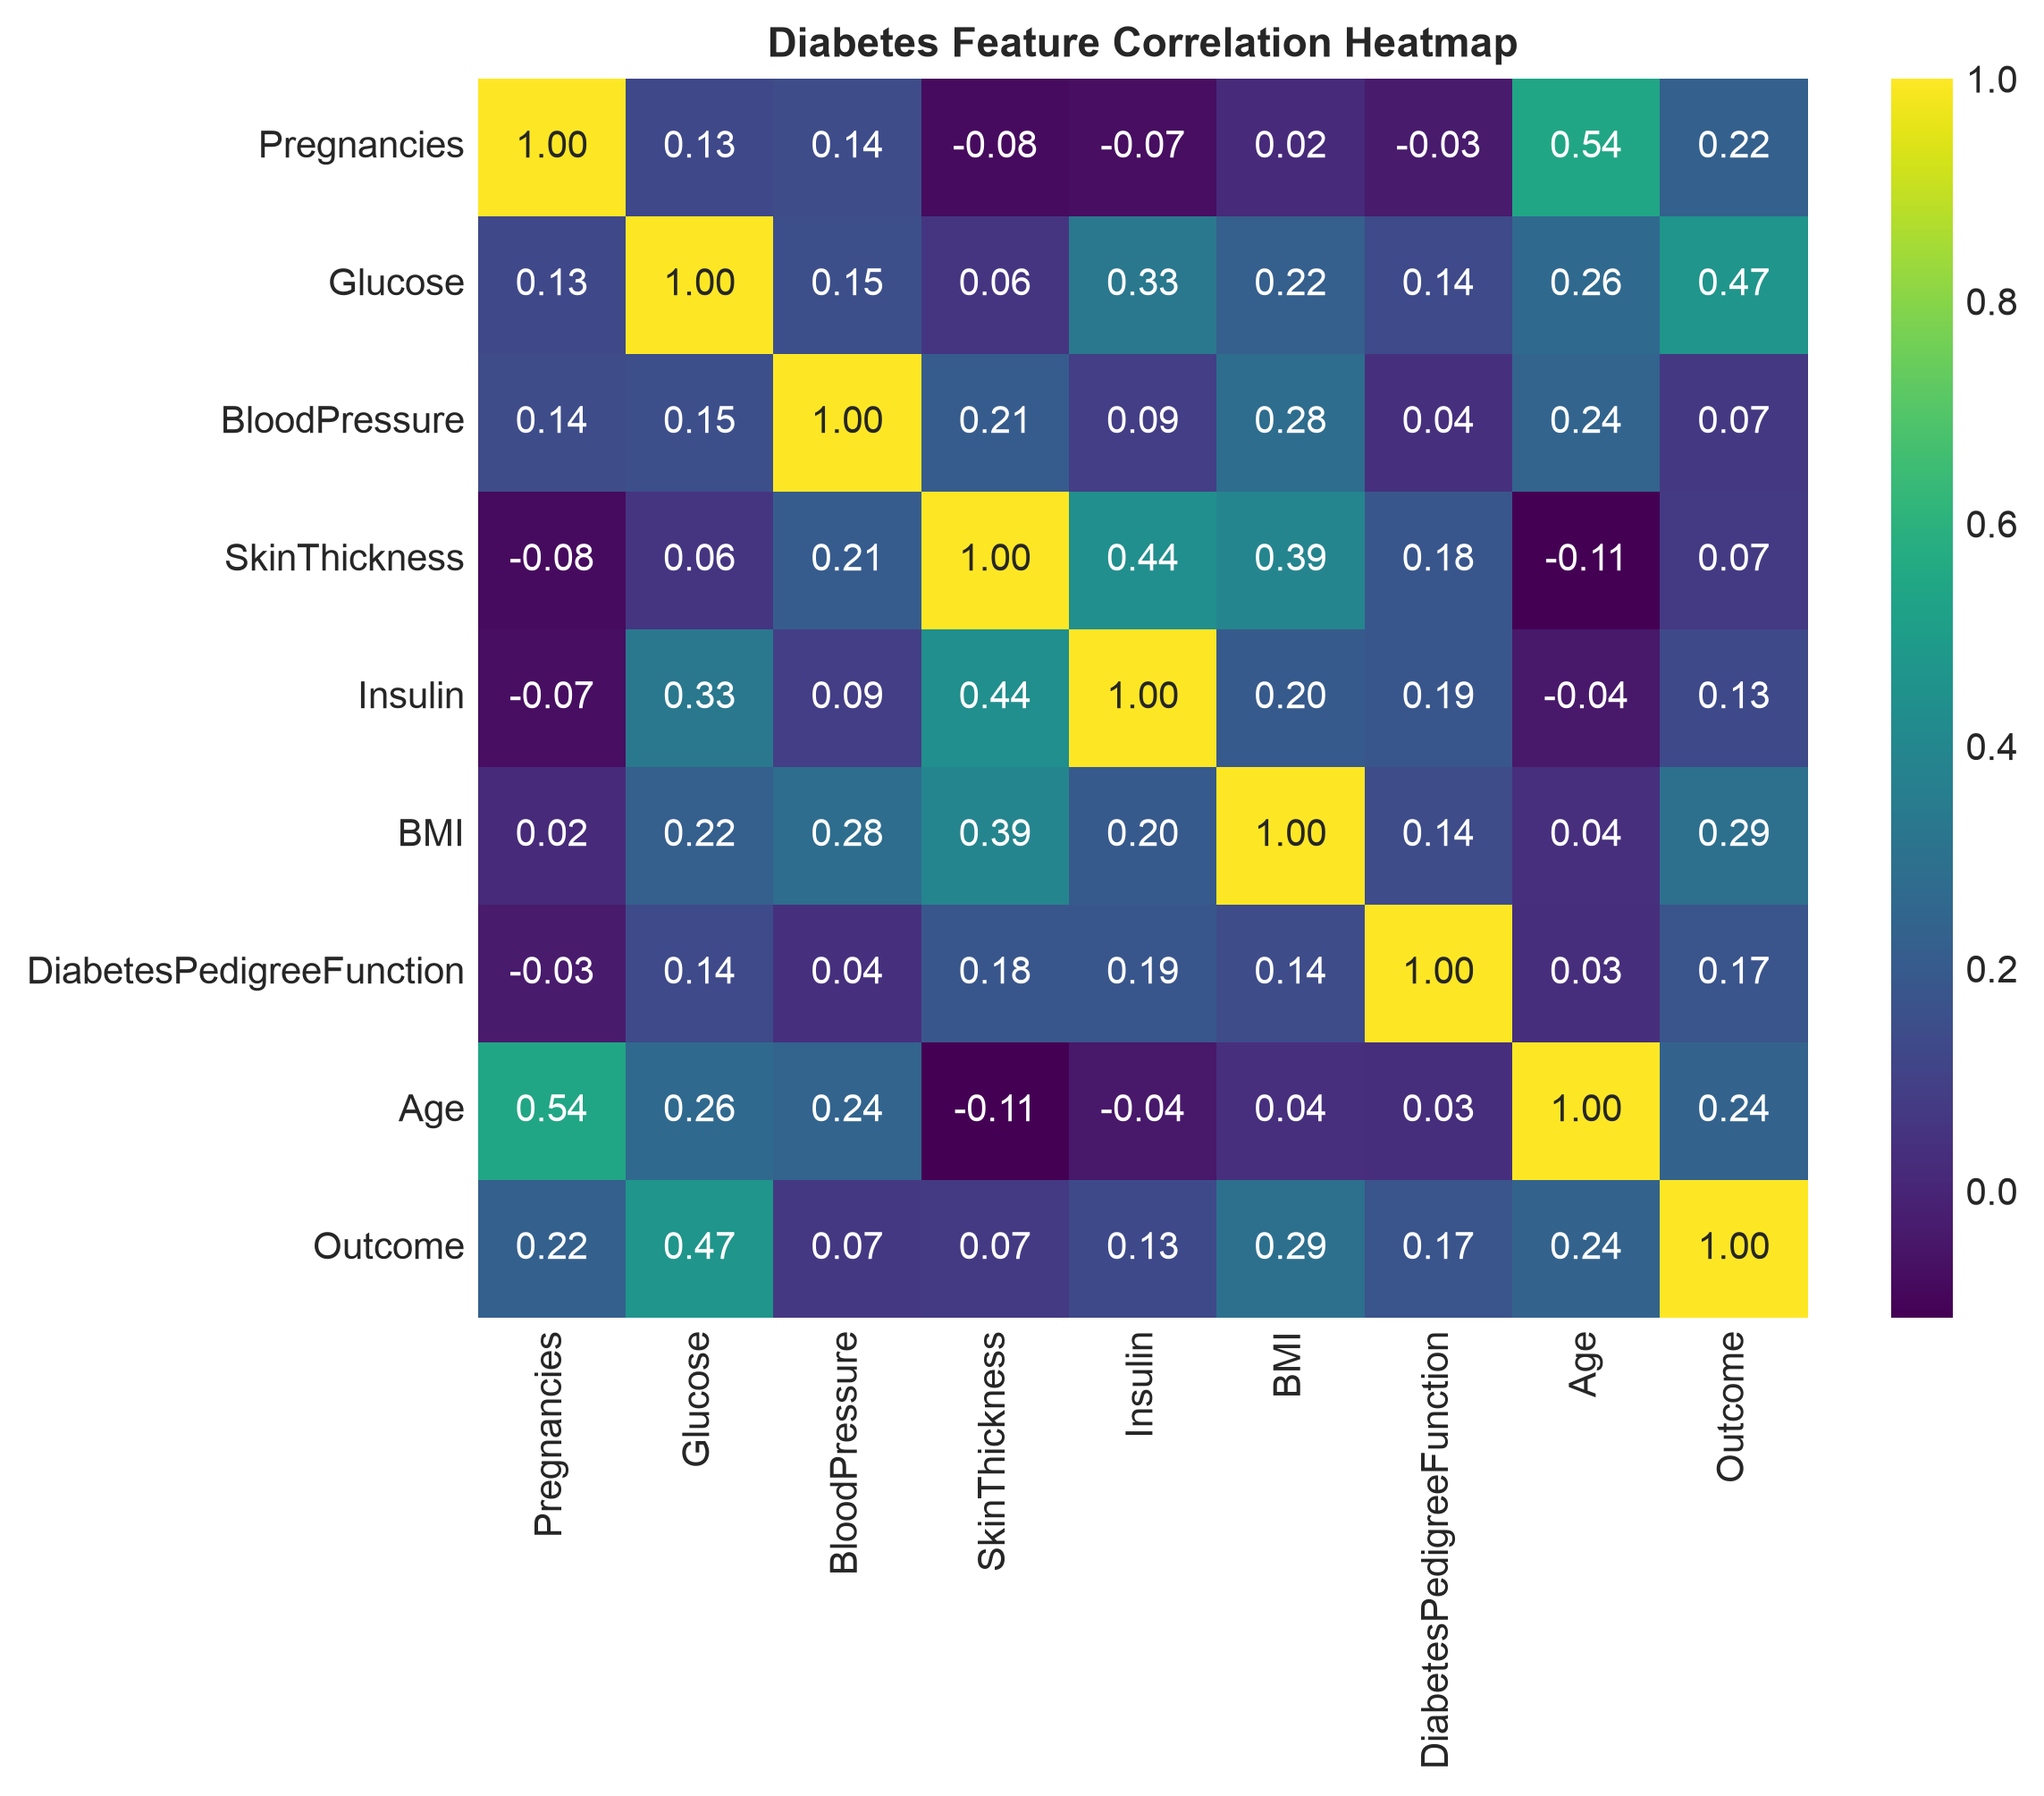
\includegraphics[width=0.7\linewidth]{images/diabetes_correlation.png}
\caption{Correlation Heatmap of Diabetes Features}
\label{fig:diab_corr}
\end{figure}

\textbf{Inference:}
\texttt{Glucose} displays the strongest positive correlation with \texttt{Outcome} ($r = 0.47$), followed by \texttt{BMI} ($r = 0.29$) and \texttt{Age} ($r = 0.24$).

\begin{figure}[H]
\centering
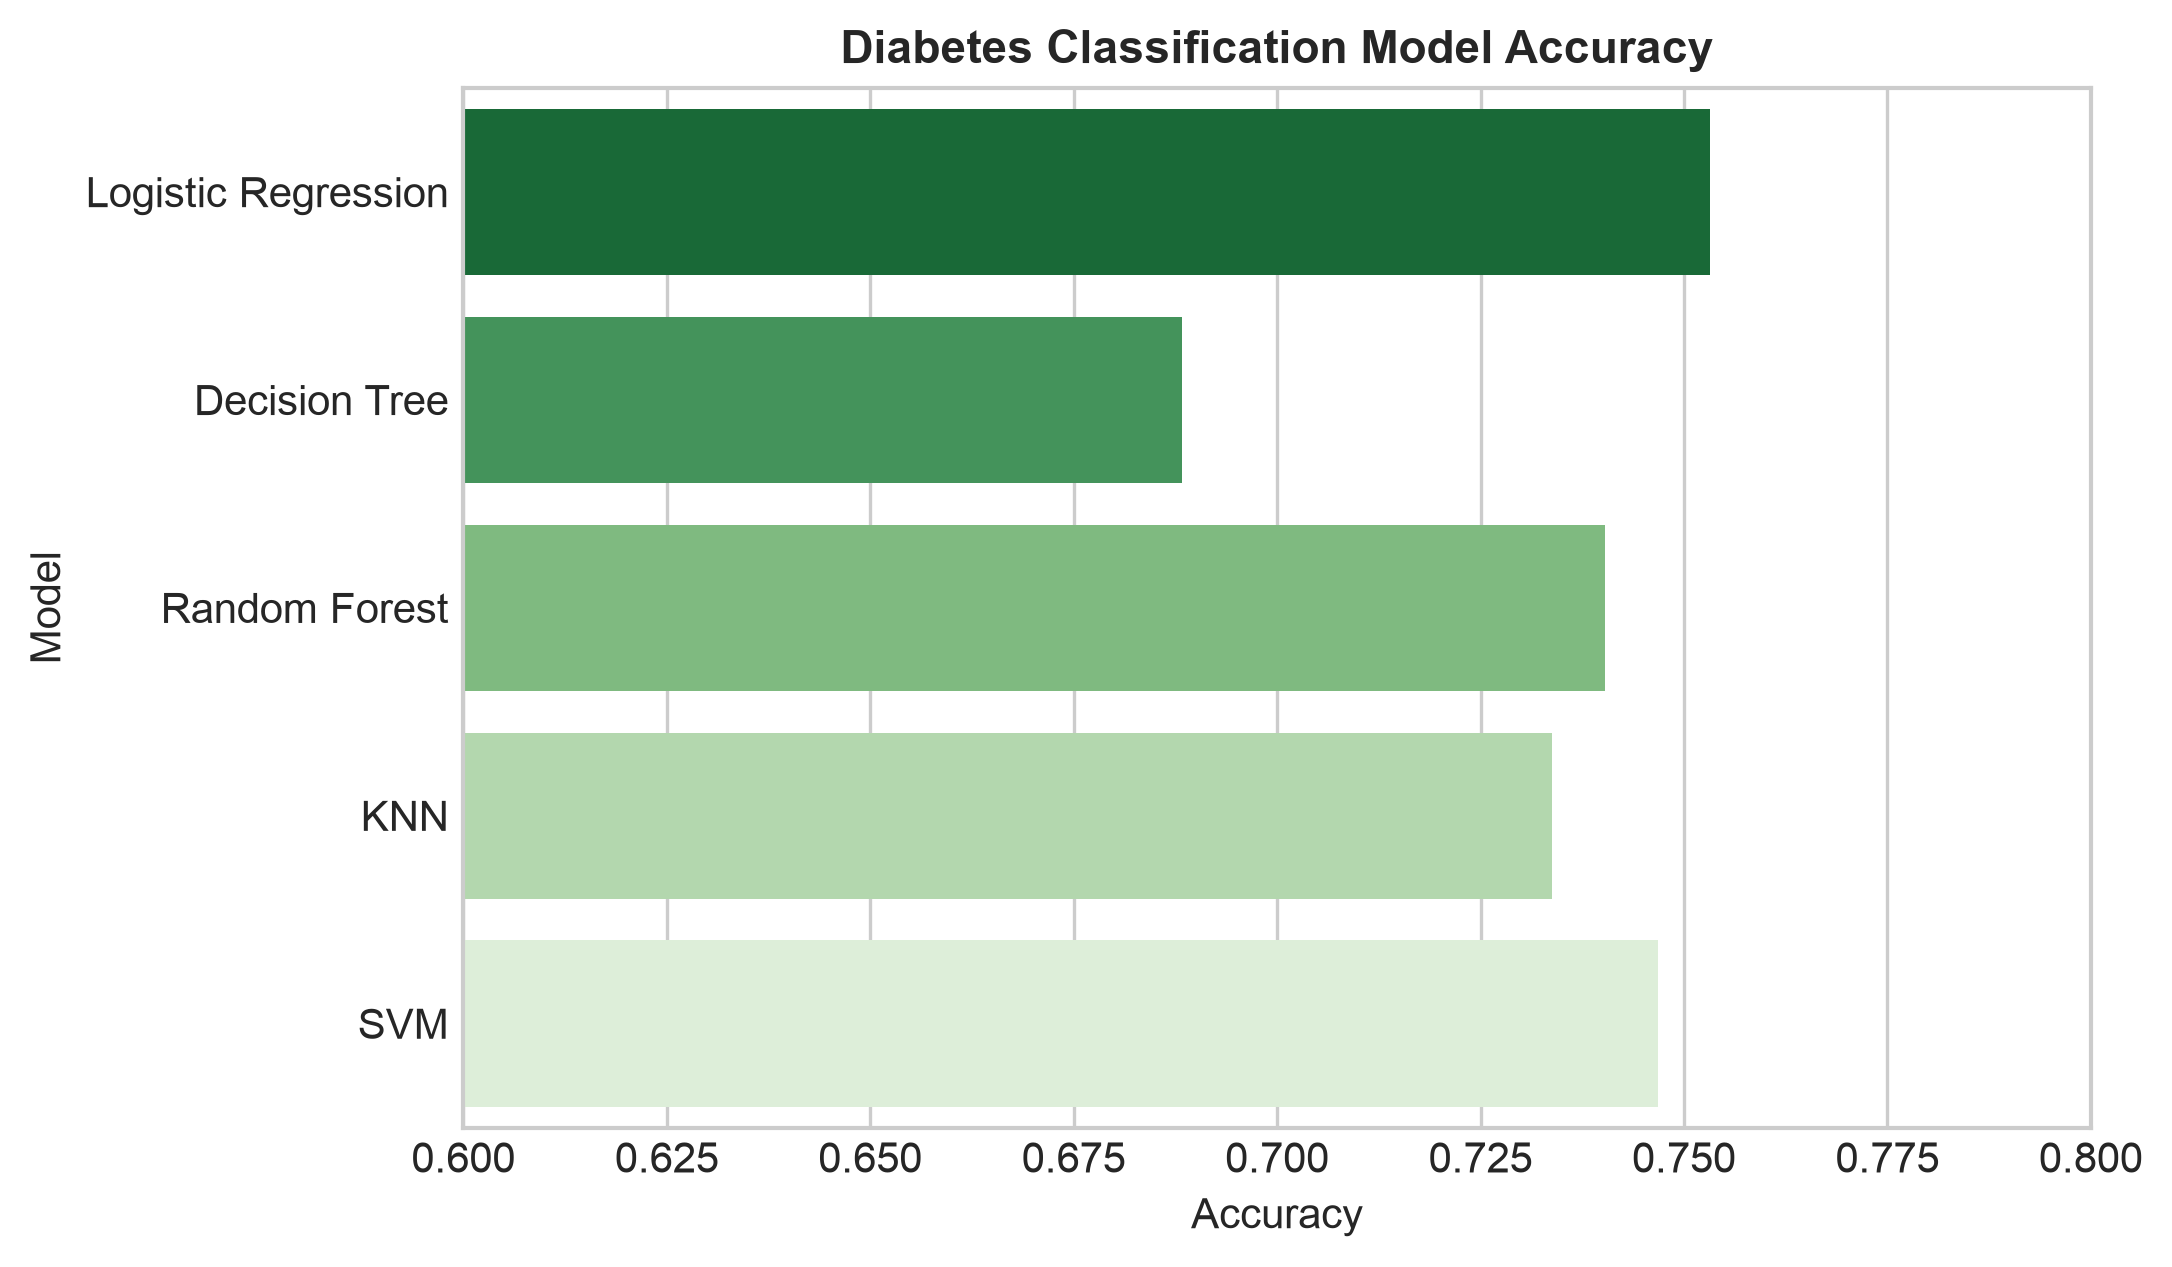
\includegraphics[width=0.7\linewidth]{images/diabetes_models_comparison.png}
\caption{Model Accuracy Comparison for Diabetes Prediction}
\label{fig:diab_comp}
\end{figure}

\textbf{Inference:}
Logistic Regression achieved the highest test accuracy of \textbf{75.32\%}, closely followed by SVM (74.68\%) and Random Forest (74.03\%).

\subsection{Data Preprocessing \& Model Evaluation}
\begin{itemize}
    \item \textbf{Preprocessing:} Replaced invalid zero values with median column statistics. Scaled features using \texttt{StandardScaler}.
    \item \textbf{Model Accuracy Breakdown:}
    \begin{itemize}
        \item \textbf{Logistic Regression: 0.7532} (75.32\%)
        \item Support Vector Machine (SVM): \textbf{0.7468} (74.68\%)
        \item Random Forest: \textbf{0.7403} (74.03\%)
        \item $K$-Nearest Neighbors (KNN): \textbf{0.7338} (73.38\%)
        \item Decision Tree Classifier: \textbf{0.6883} (68.83\%)
    \end{itemize}
\end{itemize}

\section{Case Study 5: Handwritten Character Recognition (MNIST)}

\subsection{Dataset Description \& ML Task}
The MNIST subset dataset contains $28 \times 28$ pixel grayscale images of handwritten digits (0 through 9). The task is a \textbf{Multiclass Image Classification} problem in computer vision.

\subsection{Dataset Characteristics \& Summary Statistics}
\begin{itemize}
    \item \textbf{Sample Count:} 10,000 image instances.
    \item \textbf{Feature Space:} 784 numerical pixel attributes (\texttt{1x1} to \texttt{28x28}) representing intensity values from 0 (black background) to 255 (white foreground).
    \item \textbf{Class Distribution:} Balanced across digits 0--9 ($\sim 1,000$ samples per digit class).
\end{itemize}

\subsection{Exploratory Data Analysis}

\begin{figure}[H]
\centering
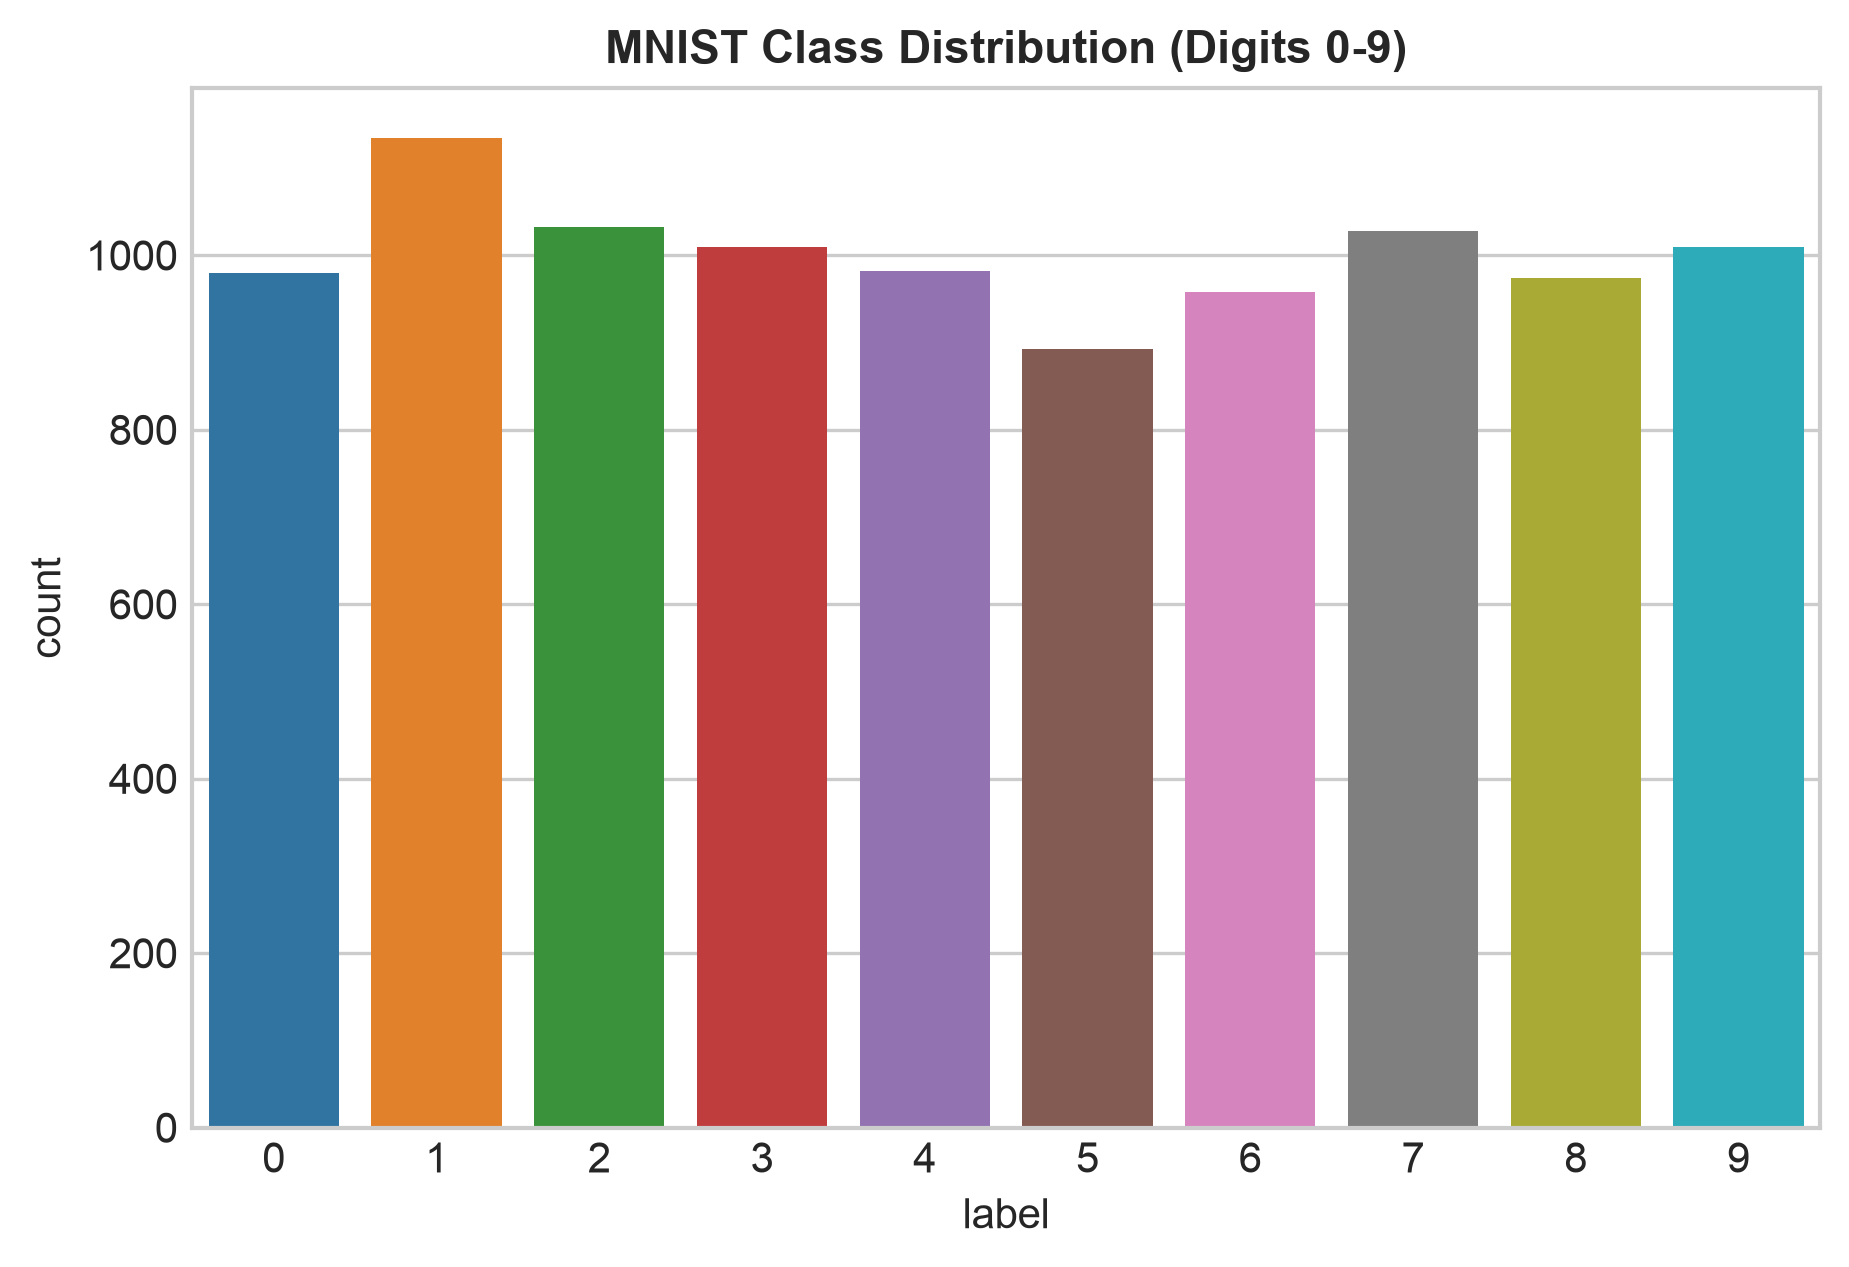
\includegraphics[width=0.7\linewidth]{images/mnist_digit_distribution.png}
\caption{Digit Label Distribution in MNIST Subsample}
\label{fig:mnist_dist}
\end{figure}

\textbf{Inference:}
The dataset is well-balanced across all 10 digit classes, avoiding majority-class bias during model training.

\begin{figure}[H]
\centering
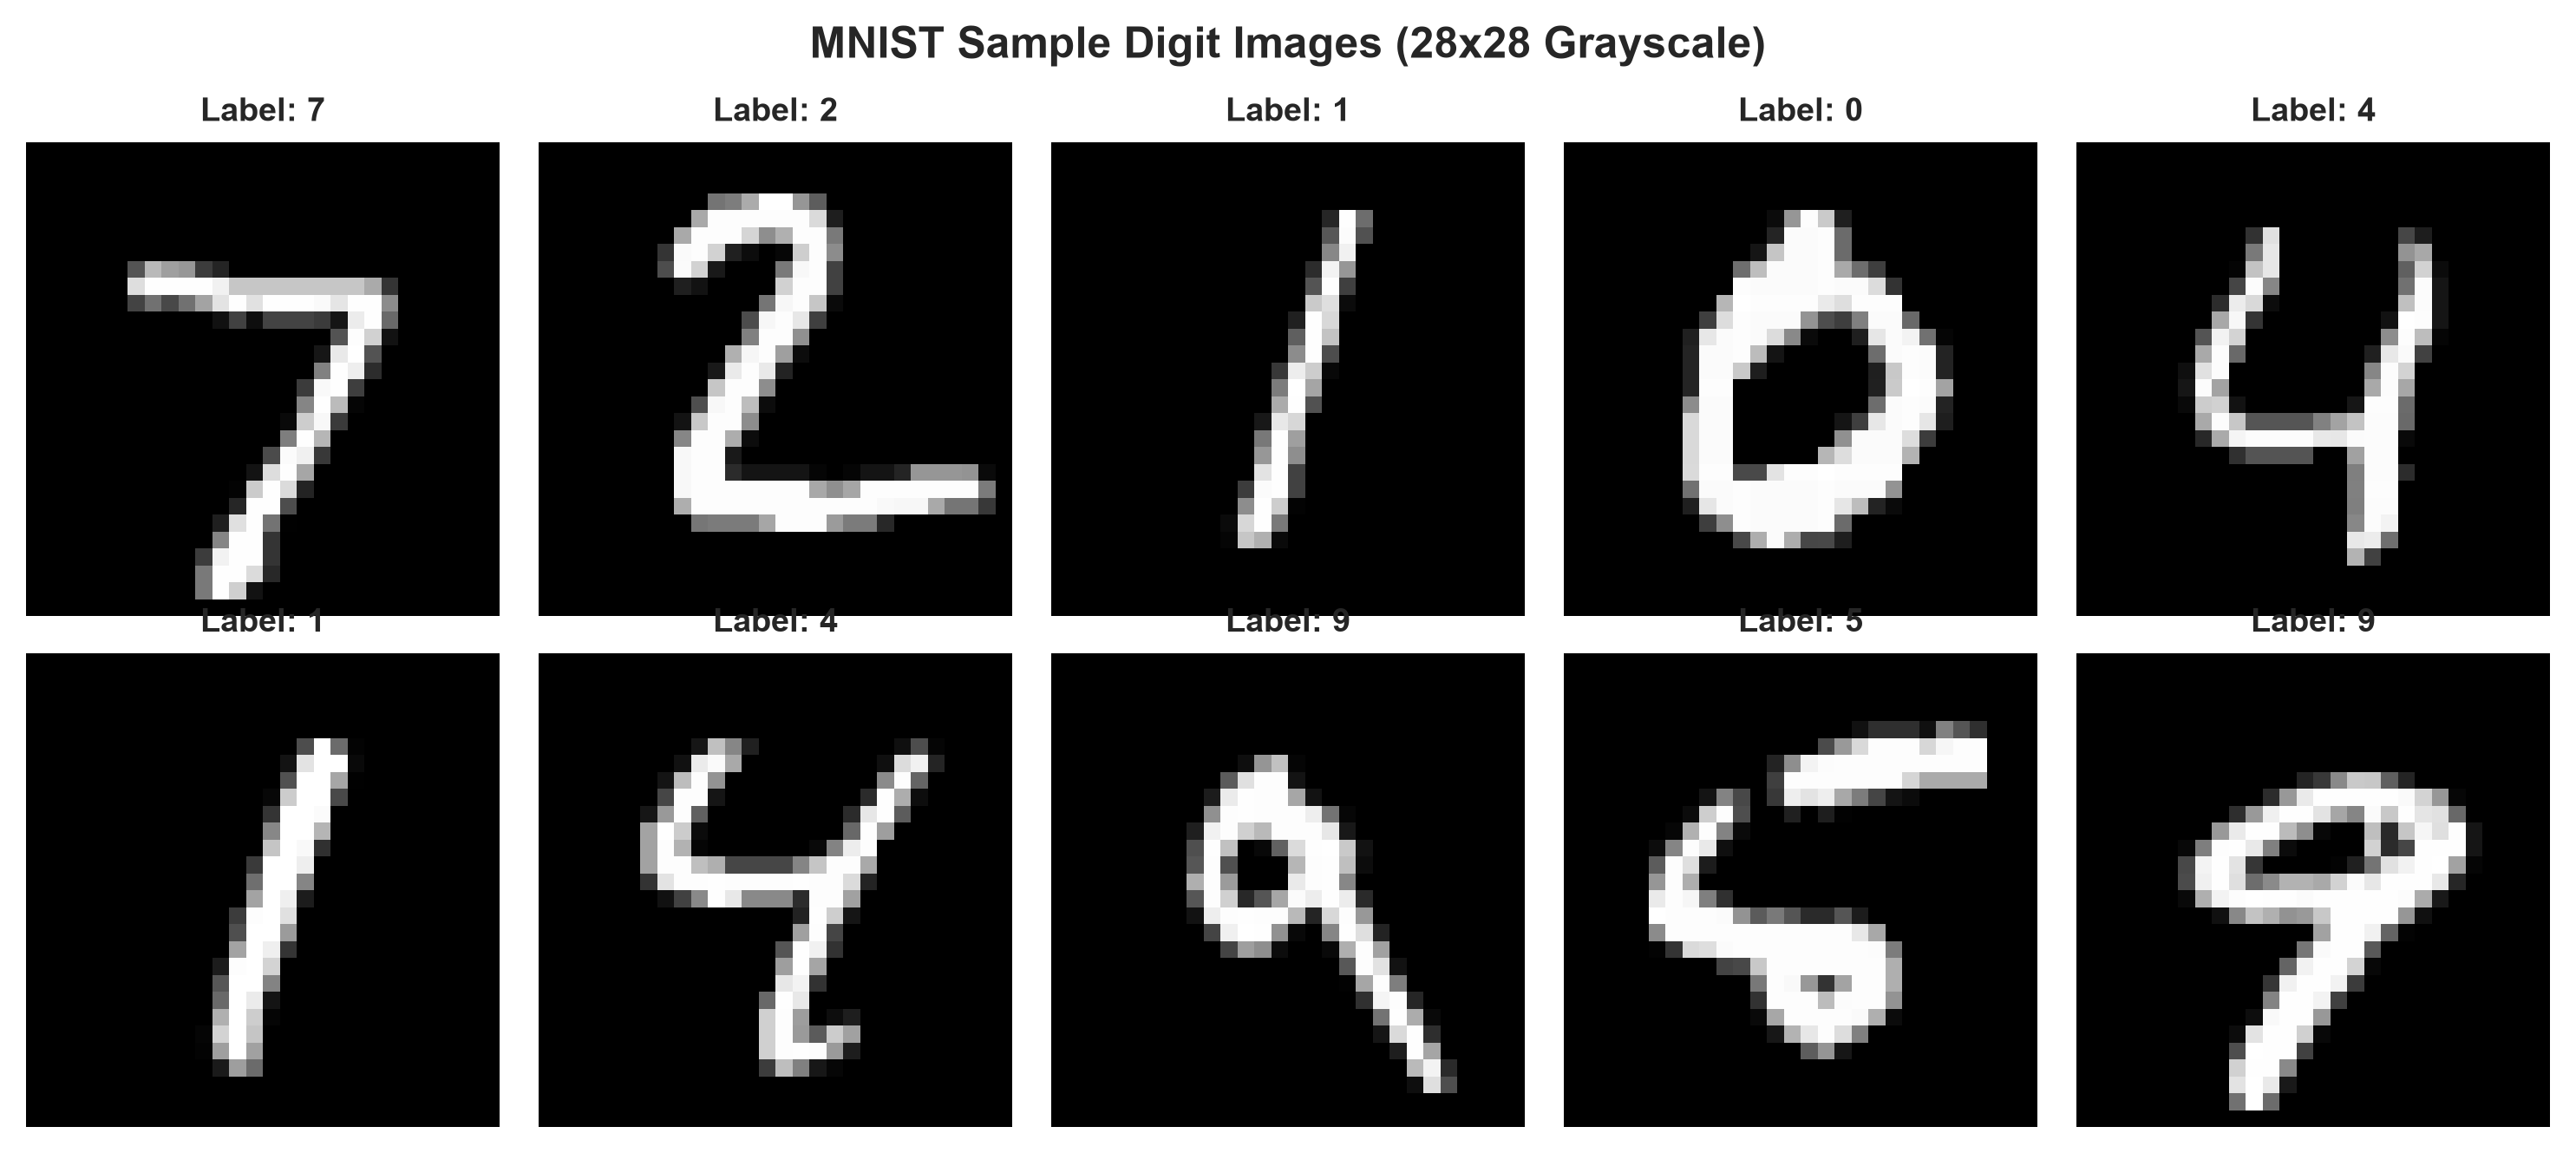
\includegraphics[width=0.85\linewidth]{images/mnist_sample_digits.png}
\caption{Sample Reconstructed $28 \times 28$ Grayscale Digit Images}
\label{fig:mnist_samples}
\end{figure}

\textbf{Inference:}
Reshaping pixel rows into $28 \times 28$ spatial grids recovers recognizable digit shapes, validating feature structure.

\begin{figure}[H]
\centering
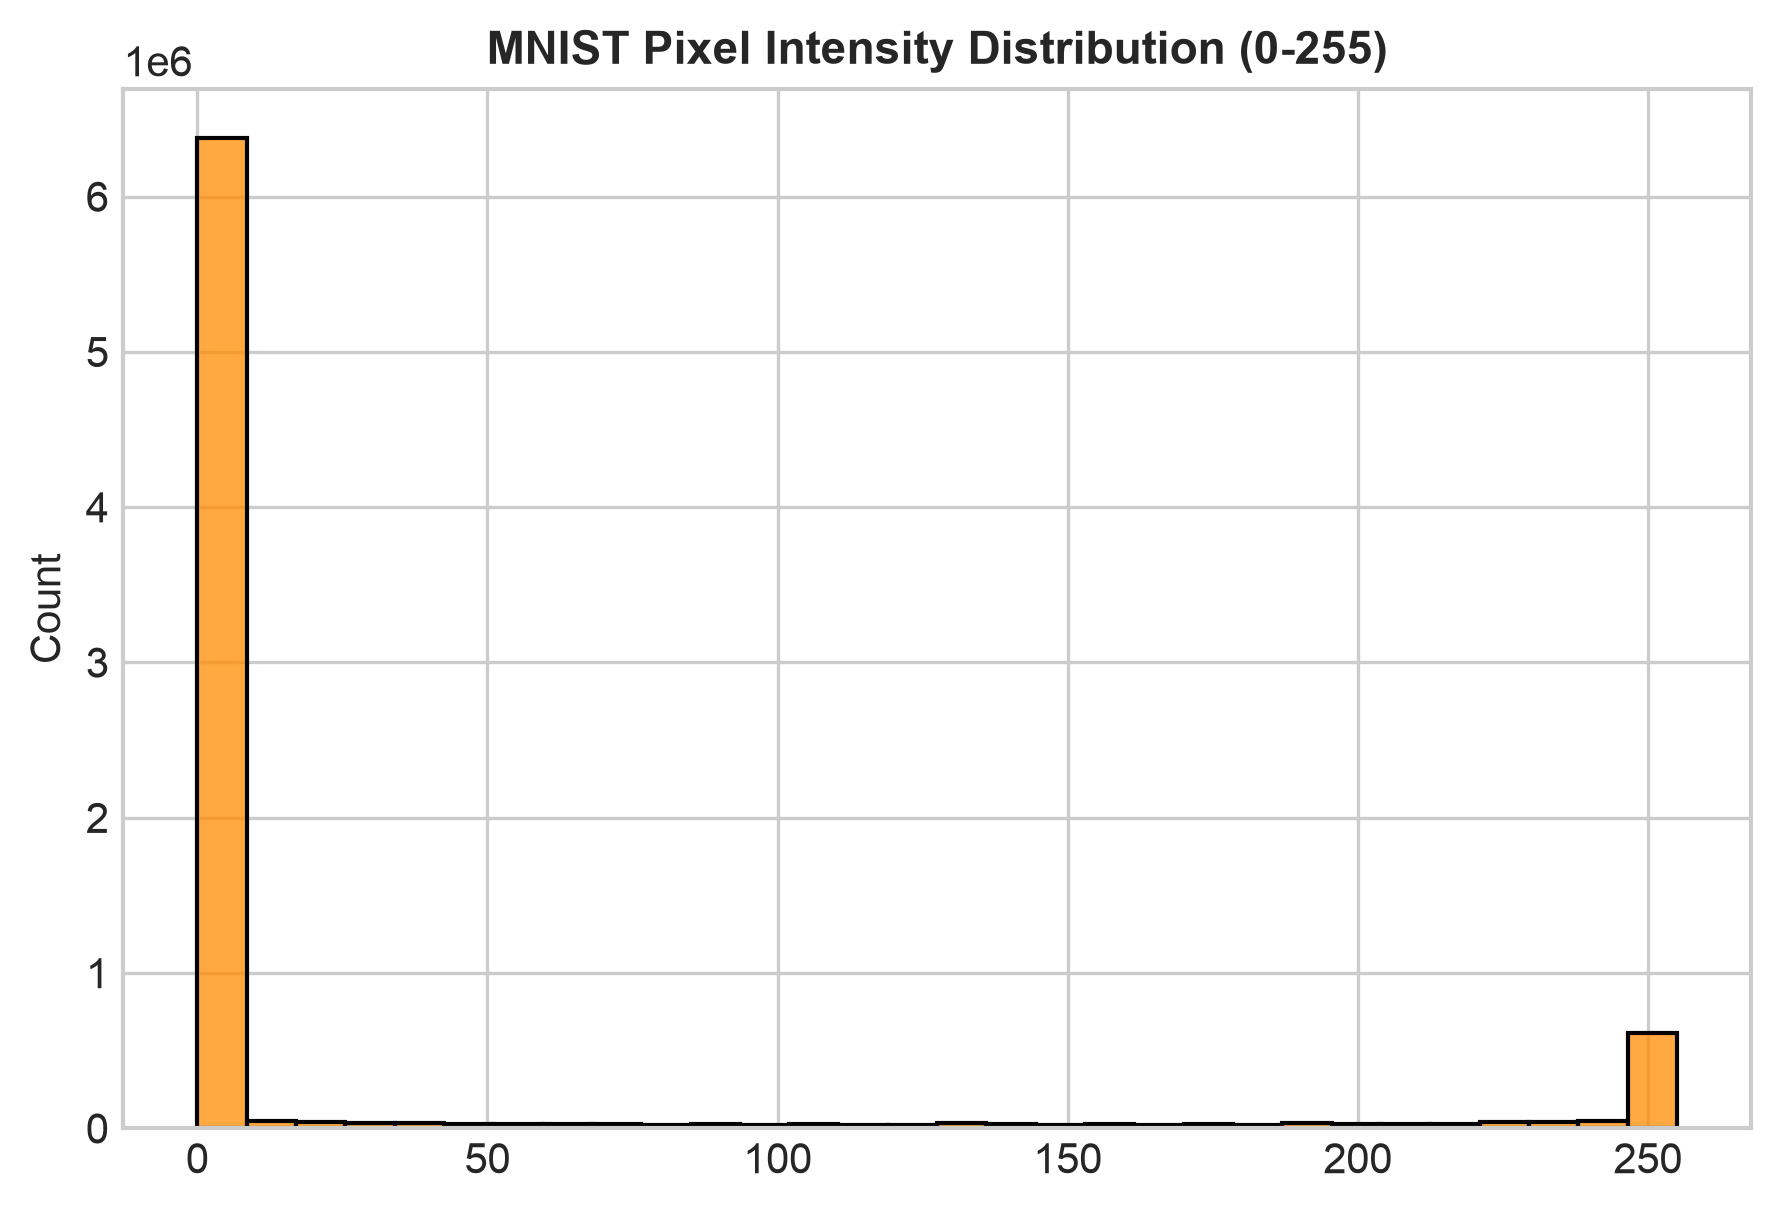
\includegraphics[width=0.7\linewidth]{images/mnist_pixel_distribution.png}
\caption{Distribution of Pixel Intensity Values}
\label{fig:mnist_pixel}
\end{figure}

\textbf{Inference:}
Pixel values exhibit a bimodal concentration at 0 (background) and 255 (stroke pixels), confirming the benefit of Min-Max normalization ($X / 255.0$).

\begin{figure}[H]
\centering
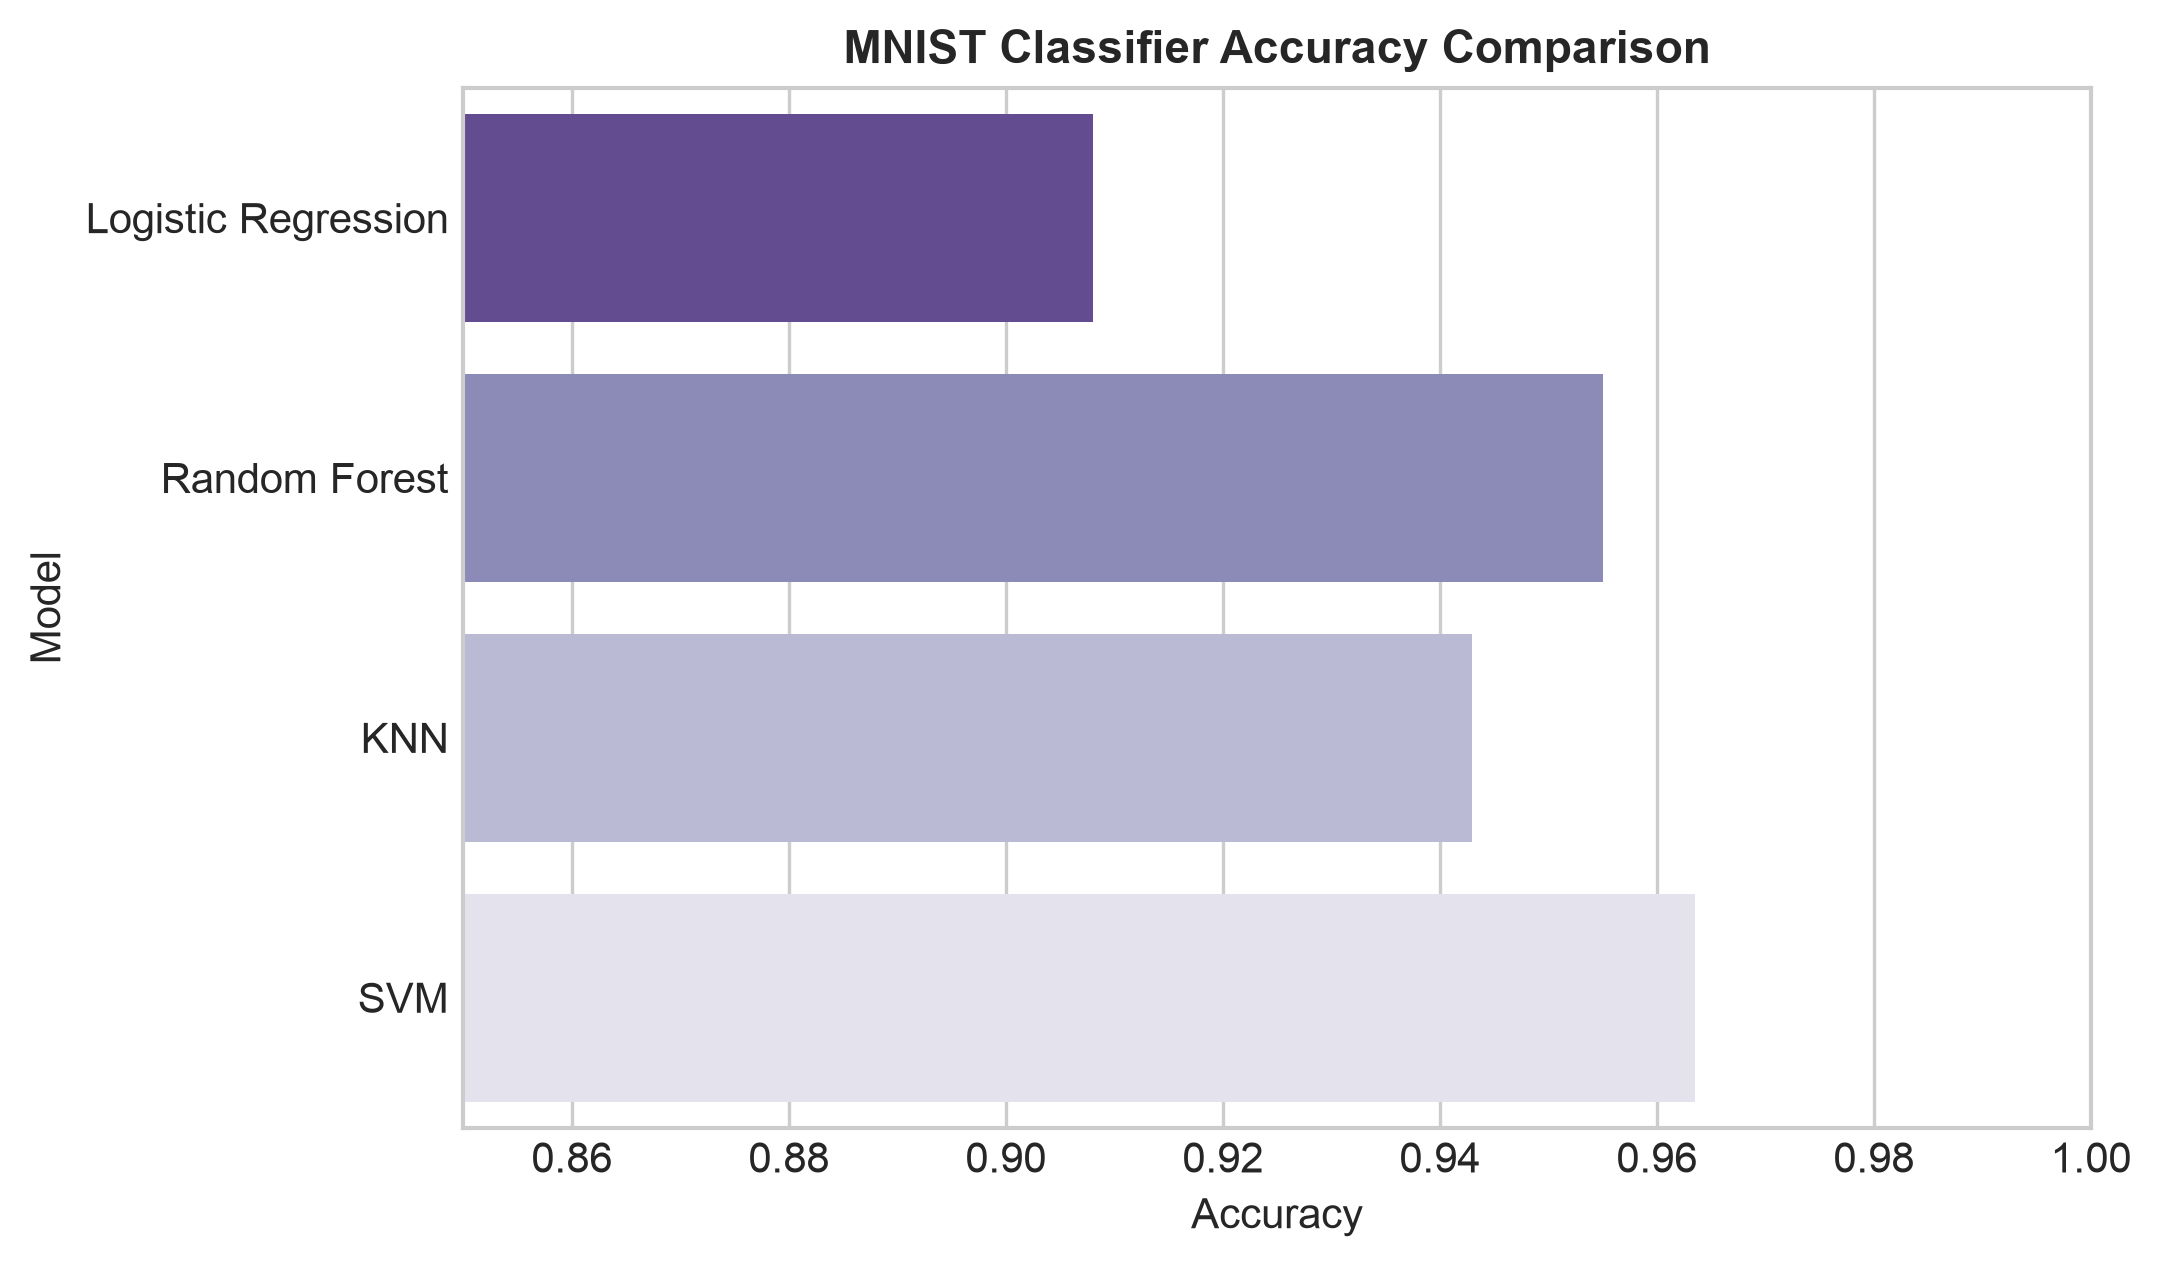
\includegraphics[width=0.7\linewidth]{images/mnist_models_comparison.png}
\caption{Accuracy Comparison of Vision Classification Models}
\label{fig:mnist_comp}
\end{figure}

\textbf{Inference:}
Support Vector Machine (RBF Kernel) achieved the top accuracy of \textbf{96.35\%}, outperforming Random Forest (95.50\%) and KNN (94.30\%).

\begin{figure}[H]
\centering
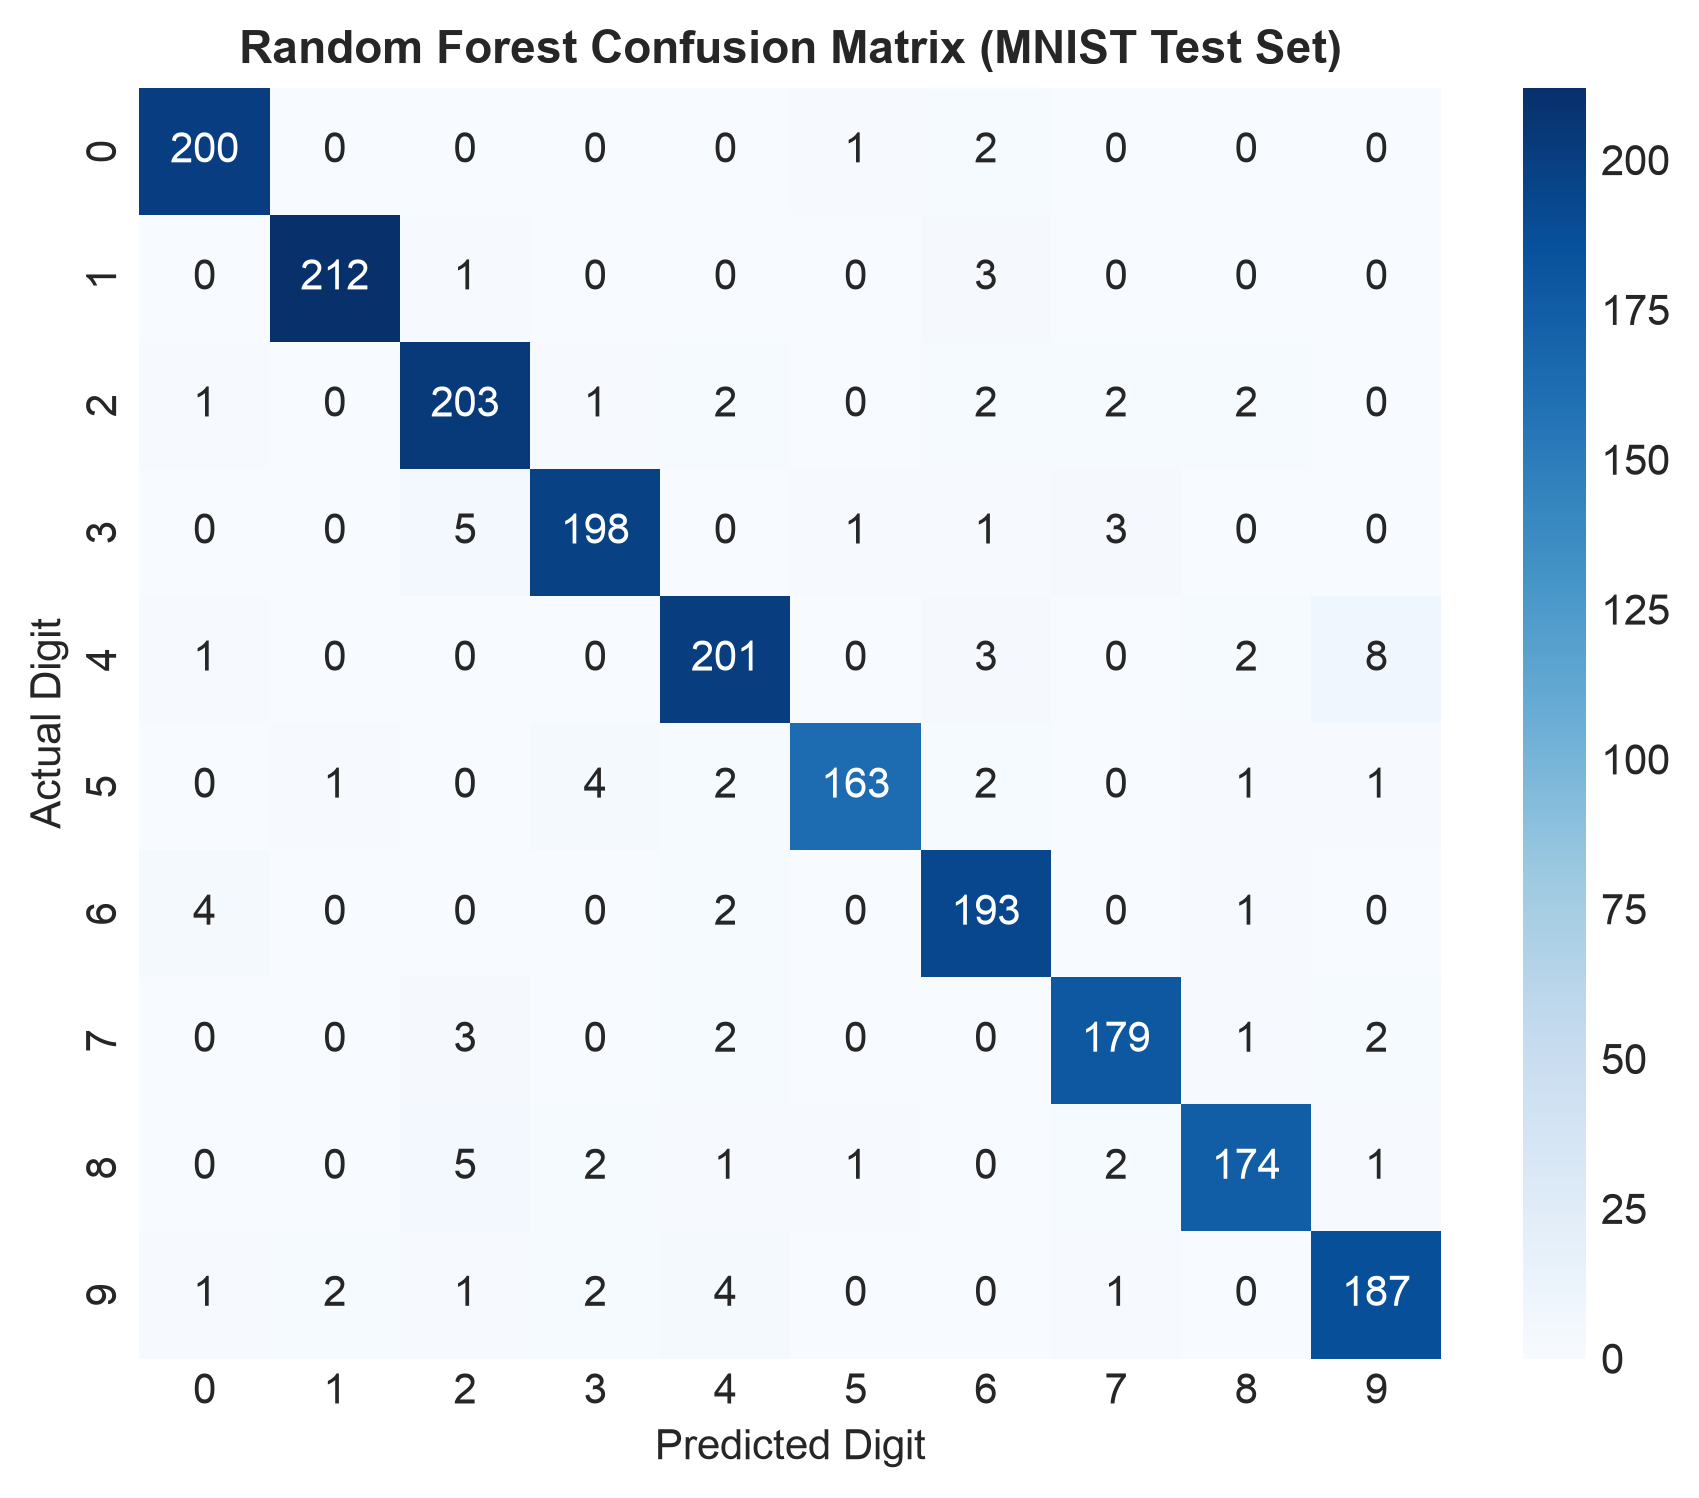
\includegraphics[width=0.65\linewidth]{images/mnist_confusion_matrix.png}
\caption{Random Forest Confusion Matrix on MNIST Test Set}
\label{fig:mnist_cm}
\end{figure}

\textbf{Inference:}
The confusion matrix demonstrates strong diagonal concentration with minor confusion between visually similar digit pairs (e.g., 4 vs. 9 and 3 vs. 8).

\subsection{Data Preprocessing \& Model Evaluation}
\begin{itemize}
    \item \textbf{Preprocessing:} Min-Max scaling ($X = X / 255.0$). 80-20 train-test split ($n_{\text{train}}=8000, n_{\text{test}}=2000$).
    \item \textbf{Model Accuracy Results:}
    \begin{itemize}
        \item \textbf{Support Vector Machine (SVM): 0.9635} (96.35\%)
        \item Random Forest Classifier: \textbf{0.9550} (95.50\%)
        \item $K$-Nearest Neighbors (KNN): \textbf{0.9430} (94.30\%)
        \item Logistic Regression: \textbf{0.9080} (90.80\%)
        \item Random Forest 5-Fold Cross Validation Mean: \textbf{0.9461} (94.61\%)
    \end{itemize}
\end{itemize}

\section{Comparative Benchmark Summary}
Table~\ref{tab:master_comparison} summarizes the machine learning task type, feature selection methodology, best algorithm, and achieved performance metric across all five datasets as required by the experiment manual.

\begin{table}[H]
\centering
\caption{Comprehensive Comparison of Machine Learning Tasks and Performance}
\label{tab:master_comparison}
\vspace{0.2cm}
\begin{tabular}{|p{3.5cm}|p{3cm}|p{3.5cm}|p{3.2cm}|p{2.2cm}|}
\hline
\textbf{Dataset} & \textbf{ML Task Type} & \textbf{Feature Engineering Technique} & \textbf{Best Performing Model} & \textbf{Primary Metric} \\ \hline
Iris Dataset & Multiclass Classification & Correlation / Pairwise Scatter Selection & Decision Tree Classifier & Accuracy: \textbf{100.0\%} \\ \hline
Loan Amount Prediction & Regression Analysis & Mode/Median Impute, One-Hot, Log Transform & Random Forest Regressor & $R^2$: \textbf{0.3228} (RMSE: 0.36) \\ \hline
Classification of Email Spam & Binary Text Classification & String Length, TF-IDF Vectorization ($K=3000$) & Support Vector Machine (SVM) & Accuracy: \textbf{97.58\%} \\ \hline
Predicting Diabetes & Binary Medical Classification & Physiological Zero Imputation, StandardScaler & Logistic Regression & Accuracy: \textbf{75.32\%} \\ \hline
Handwritten Character (MNIST) & Multiclass Vision Classification & Min-Max Pixel Scaling ($X/255$), 2D Reshaping & Support Vector Machine (SVM) & Accuracy: \textbf{96.35\%} \\ \hline
\end{tabular}
\end{table}

\section{Learning Outcomes}
Through this universal exploratory data analysis and baseline modeling experiment, the following core skills were acquired:
\begin{enumerate}
    \item Mastered key operations in \texttt{NumPy}, \texttt{Pandas}, \texttt{SciPy}, \texttt{Scikit-Learn}, \texttt{Matplotlib}, and \texttt{Seaborn} for data manipulation and visualization.
    \item Constructed an automated, reusable EDA pipeline (\texttt{perform\_EDA}) capable of handling structured tabular, text, and computer vision datasets.
    \item Implemented domain-appropriate data cleaning strategies including zero replacement for medical features, log transformation for right-skewed regression labels, and TF-IDF extraction for unstructured text.
    \item Evaluated supervised classification and regression algorithms using accuracy, precision, recall, confusion matrices, MAE, RMSE, and $R^2$ metrics.
\end{enumerate}

\section{Conclusion}
In this experiment, five distinct machine learning datasets were systematically analyzed, preprocessed, and modeled. Decision Tree achieved 100\% accuracy on Iris, SVM achieved 97.58\% on Email Spam and 96.35\% on MNIST digits, Logistic Regression led Diabetes prediction with 75.32\% accuracy, and Random Forest Regressor achieved an $R^2$ score of 0.3228 on Loan Amount prediction. The experiment demonstrates the vital role of thorough Exploratory Data Analysis and tailored preprocessing in maximizing model performance.

\section{References}
\begin{enumerate}[label={[\arabic*]}]
    \item Scikit-learn Documentation. \textit{Supervised Learning & Preprocessing Modules}. \url{https://scikit-learn.org/stable/}
    \item Pandas Development Team. \textit{Pandas API Reference & User Guide}. \url{https://pandas.pydata.org/docs/}
    \item Kaggle Datasets Repository. \textit{Predict Loan Amount, Email Spam SMS, and MNIST CSV}. \url{https://www.kaggle.com/datasets}
    \item UCI Machine Learning Repository. \textit{Iris and Pima Indians Diabetes Datasets}. \url{https://archive.ics.uci.edu/ml/}
\end{enumerate}

\end{document}
